\chapter{本地自适应差分隐私算法}

\label{ch3}

\section{引言}
与传统的集中式深度学习相比,联邦深度学习通过分布式训练在一定程度上缓解了隐私泄漏的问题。然而,许多研究表明深度学习技术可以“记忆”模型中的训练数据信息,在训练过程中,本地设备与中央服务器之间的通信信道和传递的模型参数都有可能成为第三方窃取敏感信息的途径,联邦深度学习的框架仍然存在本地训练数据泄漏等隐私威胁\upcite{ref48}。在这种情况下,敌方一旦通过白盒推理攻击或者黑盒推理攻击访问模型,就可以推演出客户端本地的训练数据。

我们认为中央参数服务器是一个"诚实但好奇"(Honest but Curious, HbC)的实体。也就是说,服务器将遵循与所有用户的协议。然而,它也试图在训练过程通过通信信道访问用户梯度,反推出关于客户端的训练数据的额外信息。出于这个原因,我们设计的本地自适应加噪算法目的是保护发送到服务器的本地梯度不会被中央服务器推断出任何关于用户的本地训练样本信息,并且尽可能维持原有模型的精度。

由于本地客户端上传至中央服务器的参数可能被敌手作为先验信息用来进行成员推理攻击,为了保护本地客户端的训练数据的隐私性,我们考虑在用户的本地模型训练阶段实现隐私保护的方案。从隐私保护的角度讲,我们只要截断了本地训练的原始输入到输出,在其中加入一道隐私保护屏障即可使最终的结果满足差分隐私。根据在哪一步截断将差分隐私保护联邦深度学习的方法分为以下几种:
\begin{itemize}
	\item \textbf{输入扰动:} 输入扰动是在获取的训练数据上直接添加噪声,之后的模型训练和优化都是基于加躁后的训练数据\upcite{ref37}\upcite{ref38}\upcite{ref39}。
	\item \textbf{输出扰动:} 输出扰动沿袭了拉普拉斯机制最简单的思路,即考虑函数输出的敏感度来添加噪声,那么在ERM公式中我们只需要考虑argmin函数输出的敏感度,基于这个敏感度来添加拉普拉斯噪声即可得到一个简单的满足差分隐私的ERM方法\upcite{ref36}。
	\item \textbf{梯度扰动:} 梯度是通过损失函数对网络模型参数进行计算得到的,其中包含了数据集的信息;在梯度上添加噪声,也能保证整体训练过程满足差分隐私。
	\item \textbf{目标扰动:} 目标扰动是在模型的目标函数中添加随机扰动,使得最终输出的结果满足差分隐私。
\end{itemize}

基于输入的扰动和输出的扰动基本可以视为一个黑盒模型,这种添加扰动的方式简单直接,但无法对模型内部数据的相关性作出细致有效的分析,在获取的训练数据和输出的训练参数上上添加过多的噪声可能会影响后续模型的收敛,破坏模型的可用性。

当前在联邦深度学习模型中应用差分隐私的主流方案是在模型的梯度上添加噪声,使输出的结果满足差分隐私并维持模型的高可用性。Song等人提出了一个$\left(\epsilon_{c}+\epsilon_{d}\right)$-差分隐私版本的随机梯度下降算法,在本地模型的每一次迭代过程中对梯度添加高斯噪声,并通过差分隐私的组合性和隐私放大效果,得到完全隐私损失的上界\upcite{ref47}。Goodfellow提出了$\ell_{2}$范式梯度裁剪的方式以限制函数敏感度,并设计了“Moments Accountant”(MA)来计算更准确的隐私预算估计\upcite{ref64},在预训练过程中,该方法与PCA相结合,形成了一个满足$\left(\epsilon_{c}+\epsilon_{d}\right)$-差分隐私的PCA。由Song等人中的实验数据可知,差分隐私随机梯度下降 (DP-SGD) 与SGD 相比严重降低了训练模型的效用。当差分隐私隐私提供的隐私强度增加时,在MNIST数据集上进行逻辑回归的训练和验证的损失率迅速增加\upcite{ref47}。在MNIST上数据集上,采用DP-SGD训练的卷积神经网络(CNN)的测试精度比SGD低得多。

在神经网络的模型训练中,不同阶段的噪声添加对于模型的准确率和收敛速度有不同的影响。在训练的初始阶段,模型的权重和最优权重的距离还很远,梯度较大,此时添加噪声对于模型的输出影响较小。随着训练的多次迭代,模型的权重越来越接近最优权重,梯度也越来越小,梯度的敏感度变高,在梯度上添加噪声对于模型输出的影响变大。之前的方案是在训练的每个阶段,在梯度上添加同样大小的噪声,会造成隐私预算的不必要损失和模型精度的降低。本文主要针对这一问题,对梯度加躁的联邦学习隐私保护方案进行改进,创新点主要有两个方面:
\begin{enumerate}
\item [(1)] 通过逐层关联传播算法计算特征对于模型输出的贡献率,根据贡献率动态地分配隐私预算,在梯度上添加自适应的高斯噪声。
\item [(2)] 根据训练轮数和梯度变化的偏差与方差动态地更新梯度裁剪阈值,对梯度进行自适应裁剪。
\end{enumerate}

\section{模型设计}
本地自适应差分隐私算法主要分为两个环节,预训练和正式训练。在预训练阶段,我们采用逐层关联传播算法在神经网络的前向传播和反向传播流程中分解模型输出,计算网络中每个神经元对模型输出的贡献率。在神经网络的正式训练阶段,通过随机梯度下降算法计算损失函数对于每个神经元的偏置和权重的梯度,基于每个神经元的贡献率给梯度分配不同的隐私预算,在梯度上添加高斯噪声。根据神经元的贡献率对梯度自适应加躁,避免了无法量化的噪声,从而提升了隐私保护模型的准确性。此外,我们根据梯度更新的统计信息对梯度裁剪阈值进行自适应调整,保证模型的快速收敛。之后我们在MNIST和FICAR-10数据集上进行实验,评估我们提出的方法,并与前人的四种差分隐私保护方案进行对比,发现我们的方法不仅产生了在模型精度方面最接近非差分隐私的模型,而且还降低了隐私预算。并且,我们针对添加本地自适应差分隐私方案的模型进行成员推理攻击,评估了该方案的隐私保护效用。

本文的模型主要针对本地设备的模型训练阶段,设计自适应的梯度加躁和裁剪算法,保证中央服务器接收到满足$(\epsilon, \delta)$-差分隐私的权重,从而减轻成员推理攻击对联邦学习所构成的隐私威胁。本地客户端进行模型训练的基本流程如图\ref{fig:自适应差分隐私SGD算法流程图}所示,通过从数据集D中随机采样构造各批次的样本,对于每一批样本通过梯度下降算法进行模型训练,通过梯度自适应裁剪算法加快模型的收敛速度,在梯度上添加自适应的高斯噪声,使整体训练系统满足$(\epsilon, \delta)$-差分隐私。

\begin{figure}[!hbt]
\centering
	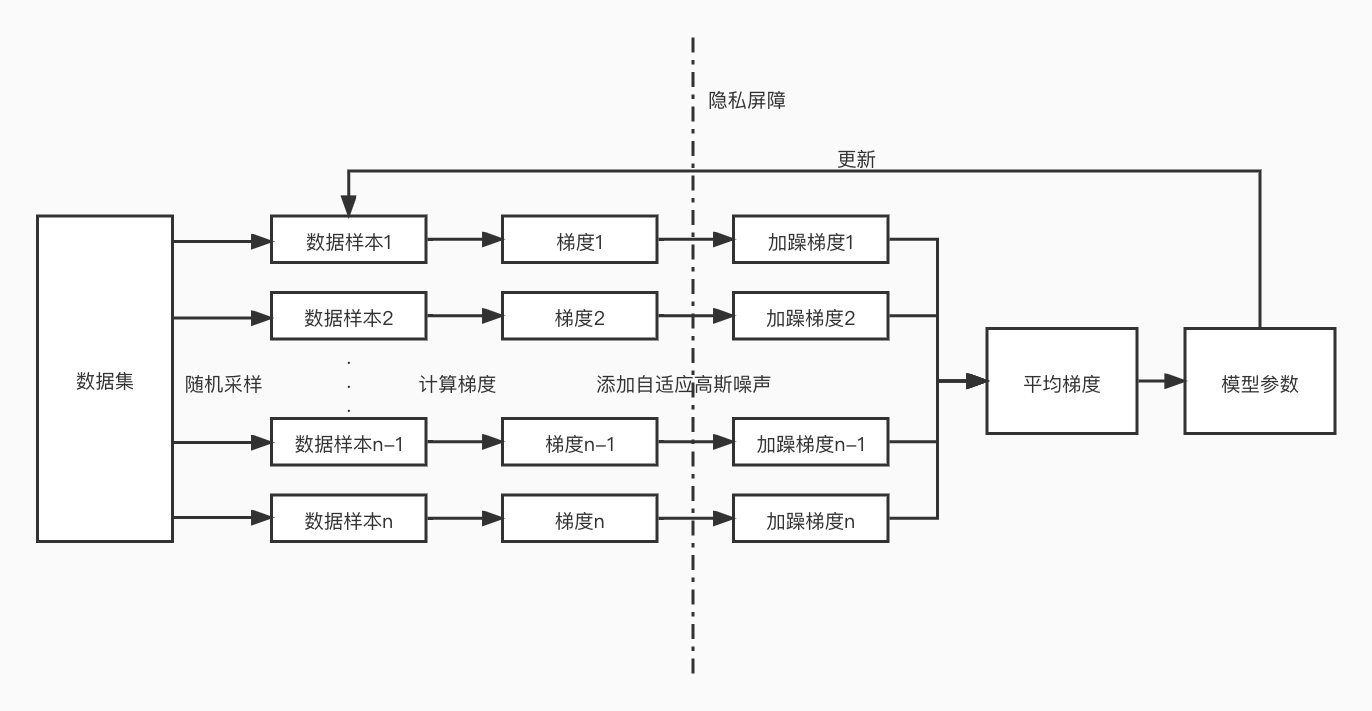
\includegraphics[scale=0.2]{fig2/C3/自适应差分隐私流程图}%联邦学习的系统架构
	\caption{自适应差分隐私SGD算法流程图}
	\label{fig:自适应差分隐私SGD算法流程图}	
\end{figure}

\subsection{梯度的自适应加躁算法}
% 在第二章我们详细介绍了联邦学习的流程和神经网络的结构,每个用户在本地设备的私有数据集上进行训练。本地训练的流程主要概括为前向传播和反向传播。神经网络中前向传播算法的第一步在输入层,我们使用前馈神经网络接收输入的$x$运行前向传播算法,得到预测值,然后通过反向传播算法不断调整参数使与预测值和真实值之间的误差降低。

Bach等人提出了针对神经网络的逐层关联传播算法\upcite{ref65},这是一种用于计算特定图像区域对分类器输出结果影响的技术。该技术被认为是非常有效的,可以逐个像素地分解图像的预测值\upcite{ref76},可以应用在深度神经网络中对各神经层进行循环重正化\upcite{ref77},用来分解深度神经网络的预测值,得到神经网络中各个特征对于模型结果的贡献。经典的反向传播算法是通过链式法则对模型的输出进行反向求导,根据损失函数计算每个神经元对模型总误差的贡献值,然后来调整模型的权重,以降低总误差。根据这一思路,在本文的工作中,创造性地利用逐层关联传播算法将神经网络的输出值按层进行分解,得到每层的神经元对于模型输出的贡献率。为了尽量弥补噪声添加而带来的模型可用性下降的问题,我们根据特征对于模型输出的总体影响,分配隐私预算。在贡献率大的特征上分配较高的隐私预算,添加的噪声量较小;在贡献率较低的特征上分配较低的隐私预算,添加的噪声量较大。

本地用户进行模型训练的主要步骤如下:
\begin{enumerate}
\item [(1)] 对模型进行预训练,运行逐层关联传播算法计算每个神经元对于模型输出的归因分数,归因分数代表了神经元对于模型输出的贡献程度;
\item [(2)] 初始化神经网络的参数$\theta_{0}$、模型训练的迭代次数$T$、高斯噪声隐私参数$\sigma$
\item [(3)] 从数据集D中随机采样$L$训练样本送入神经网络中,运行前向传播算法,得到模型的预测结果$f_{X_{i}}\left(\theta_{t}\right)$
\item [(4)] 通过交叉熵损失函数计算模型的预测值$f_{X_{i}}\left(\theta_{t}\right)$与真实值$\mathrm{y}_{\mathrm{i}}$之间的误差$\mathcal{L}\left(\theta_{t}, X_{i}\right)=-\sum_{\left(X_{i}, y_{i}\right) \in L_{i}} y_{i} \log f_{X_{i}}\left(\theta_{t}\right)$,运行反向传播算法,计算损失函数对于所有神经元的权重和偏置的梯度$\mathbf{g}_{t}\left(x_{i}\right)$
\item [(5)] 根据步骤(1)中计算的归因分数,进行隐私预算的分配,计算每个梯度分配到的隐私预算$\sigma_{i}=\frac{\sigma_{t}}{\ddot{Cr_{j}}\left(x_{i}\right)}$
\item [(6)] 根据隐私预算在梯度上添加对应的高斯噪声
\item [(7)] 重复步骤(3)-(7)直至模型收敛,输出模型权重
\end{enumerate}

\subsubsection{神经元归因分数的计算}
在卷积神经网络结构中,每个隐藏神经元的转化过程表示为$y=\sigma(\mathbf{x} * \omega+b)$,其中$\mathbf{x}$代表输入向量,$y$是输出,$b$和$\omega$分别代表{}偏置项和权重矩阵。$\sigma()$是一个激活函数,用于结合线性变换和非线性变换。在前向传播过程中,图像输入以像素的形式进入网络,然后与网络权重w相乘,再加上一个偏置b,并通过激活函数使其成为非线性计算,这个过程一直持续到输出层得到模型输出。

对于卷积神经网络等网络结构,模型输出表示为$F_{\theta}$,输出层的神经元表示为$z$。在逐层关联传播算法中,根据神经网络的结构自前向后计算总归因分数$Cr_{z}$。输出层的归因分数通常作为输出层的预激活值,在反向传播过程中,每一层的所有神经元的归因分数总和是恒定。运行前向传播算法获得总归因分数后利用$F_{\theta}$和$Cr_{z}$在反向传播算法中逐层分解,计算各层神经元的归因分数,它代表了每个神经元对于模型输出的贡献程度。

\begin{figure}[!hbt]
\centering
	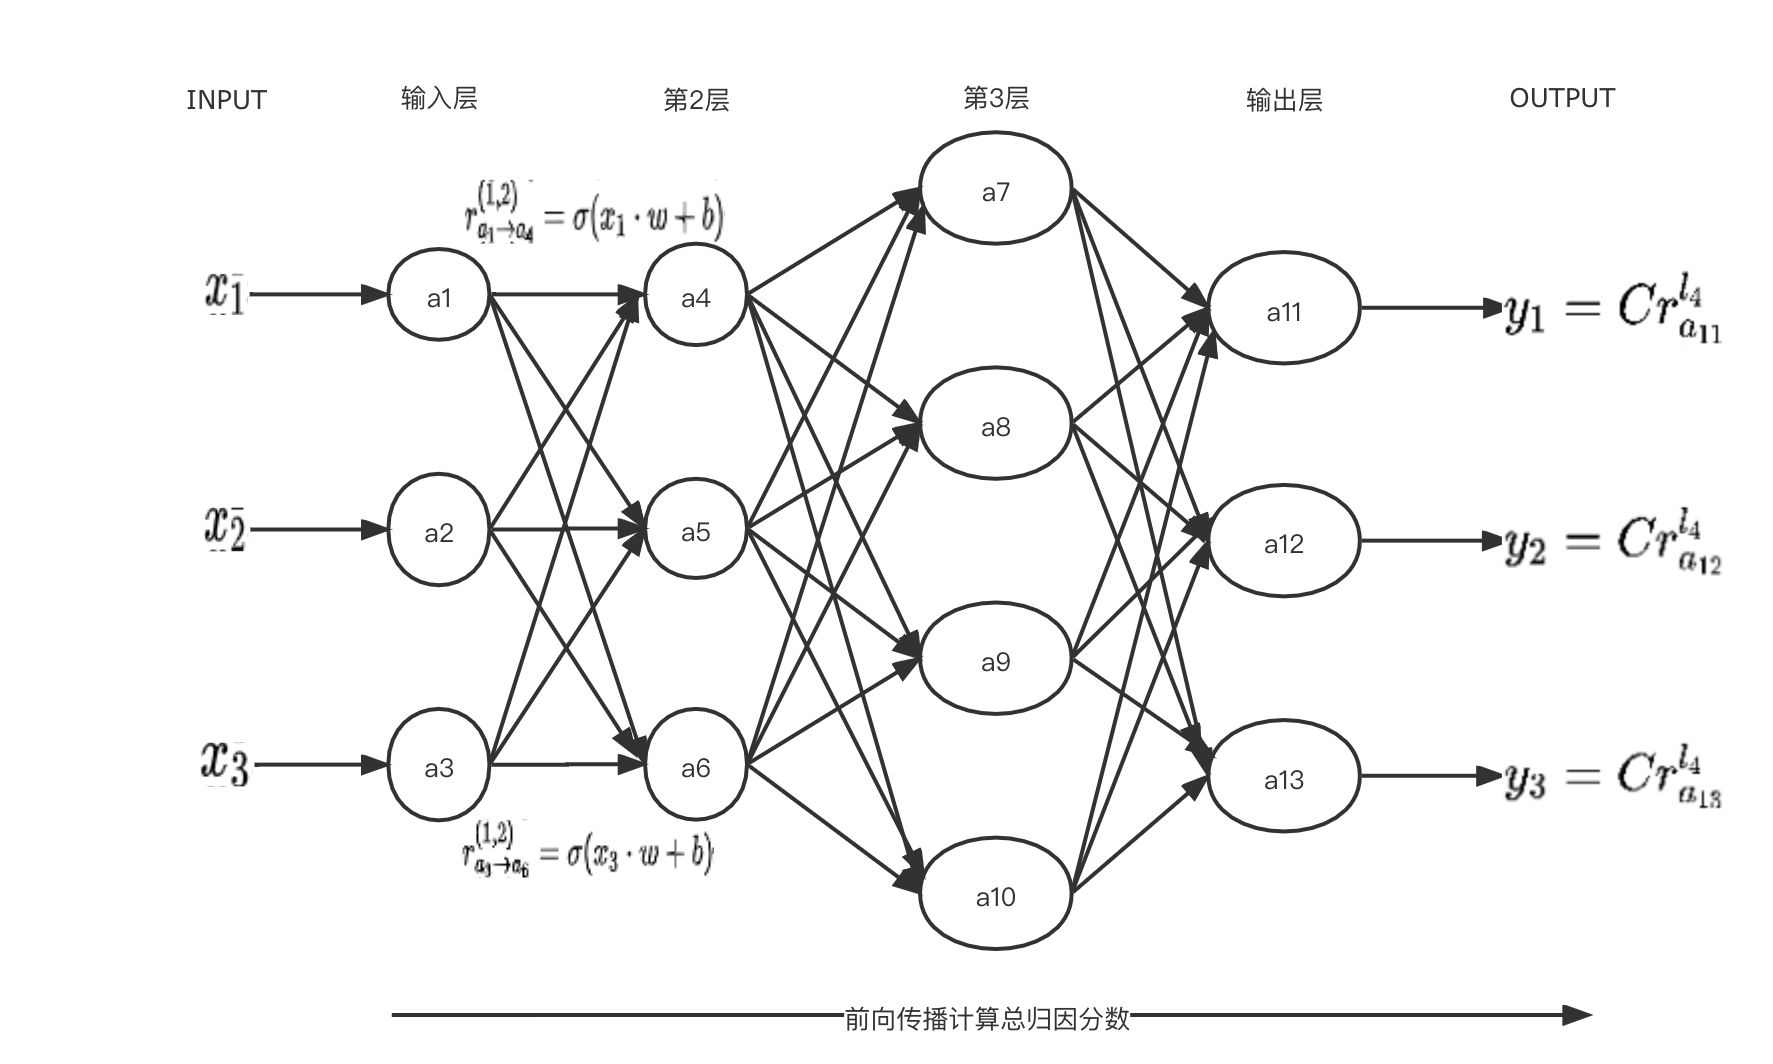
\includegraphics[scale=0.25]{fig2/C3/自适应-前向传播}%联邦学习的系统架构
	\caption{逐层关联传播算法:根据前向传播计算总归因分数}
	\label{fig:逐层关联传播算法:根据前向传播计算总归因分数}	
\end{figure}

我们具体阐述如何计算网络中某一个神经元$a_{j}$的归因分数。箭头$(\rightarrow)$和$(\leftarrow)$分别代表第$l_{m}$层和第$l_{m+1}$层的前向连接和反向连接关系, $r_{n \rightarrow z}$表示由神经元n到神经元z的前向传播关系,$R_{n \leftarrow z}^{(l_{m}, l_{m+1})}$表示第m+1层的神经元z到第m层的神经元n的反向传播关系。在前向传播算法中,神经元$a_{i1}$接受上一层输入的像素值 $x_{1}$并计算$r_{a_{i1} \rightarrow a_{j}}^{(l_{m}, l_{m+1})}=\sigma\left(x_{1} * \omega+b\right)$,然后将计算结果传输给第$l_{m+1}$层的神经元$a_{j}$;同理,输出层$l_{m+1}$的神经元$a_{j}$接受来自上一层神经元$a_{i2}$的计算结果$r_{a_{i2} \rightarrow a_{j}}^{l_{m}, l_{m+1}}=\sigma\left(x_{2} * \omega+b\right)$,那么模型输出的结果为$r_{a_{j}}=r_{a_{i1} \rightarrow a_{j}}+r_{a_{i2} \rightarrow a_{j}}+b_{a_{j}}$。如图\ref{fig:逐层关联传播算法:根据前向传播计算总归因分数}所示,神经元$a_{4}$接收来自输入层的神经元$a_{1}$、$a_{2}$、$a_{3}$的计算结果,分为别$\sigma\left(x_{1} * \omega+b\right)$、$\sigma\left(x_{2} * \omega+b\right)$、$\sigma\left(x_{3} * \omega+b\right)$,神经元$a_{4}$接收的总输入值为$r_{a_{1} \rightarrow a_{4}}^{(l_{1}, l_{2})}+r_{a_{2} \rightarrow a_{4}}^{(l_{1}, l_{2})}+r_{a_{3} \rightarrow a_{4}}^{(l_{1}, l_{2})}+b_{a_{4}}$。

$C r_{a_{i}}^{l_{m}}\left(x_{i}\right)$表示第$m$层的神经元 $a_{i}$对于模型输出的归因分数。因为输出层的神经元的归因分数等于模型的输出,对于图\ref{fig:逐层关联传播算法:根据前向传播计算总归因分数}中的神经元$a_{11}$,有$C r_{a_{11}}^{l_{4}}\left(x_{i}\right)=y_{1}$。

根据神经网络相邻层间的线形关系和反向传播算法,第m层神经元和第m+1层神经元的反向关联性表示为:
$$
R_{a_{i} \leftarrow a_{j}}^{(l_{m}, l_{m+1})}=\left\{\begin{array}{l}\frac{r_{a_{i}  \rightarrow a_{j} }}{r_{a_{j}}+b_{a_{i}}} \cdot C r_{a_{j}}^{l_{m} }, r_{a_{j}} \geq 0 \\ \frac{r_{a_{i} \rightarrow a_{j} }}{r_{a_{j} }-b_{a_{i}}} \cdot C r_{a_{j}}^{l_{m} }, r_{a_{j}}<0\end{array}\right.
$$


第m层的神经元$a_{i}$的归因分数$Cr_{a_{i}}^{l_{m}}\left(x_{i}\right)$即为与之相关联的第$m+1$层的所有神经元${a_{j}\in l_{m+1}}$的归因分数总和:
$$
Cr_{a_{i}}^{l_{m}}\left(x_{i}\right)=\sum_{a_{j} \in l_{m+1}} Cr_{a_{i} \leftarrow a_{j}}^{l_{m} \leftarrow l_{m+1}}\left(x_{i}\right)
$$

\begin{figure}[!hbt]
\centering
	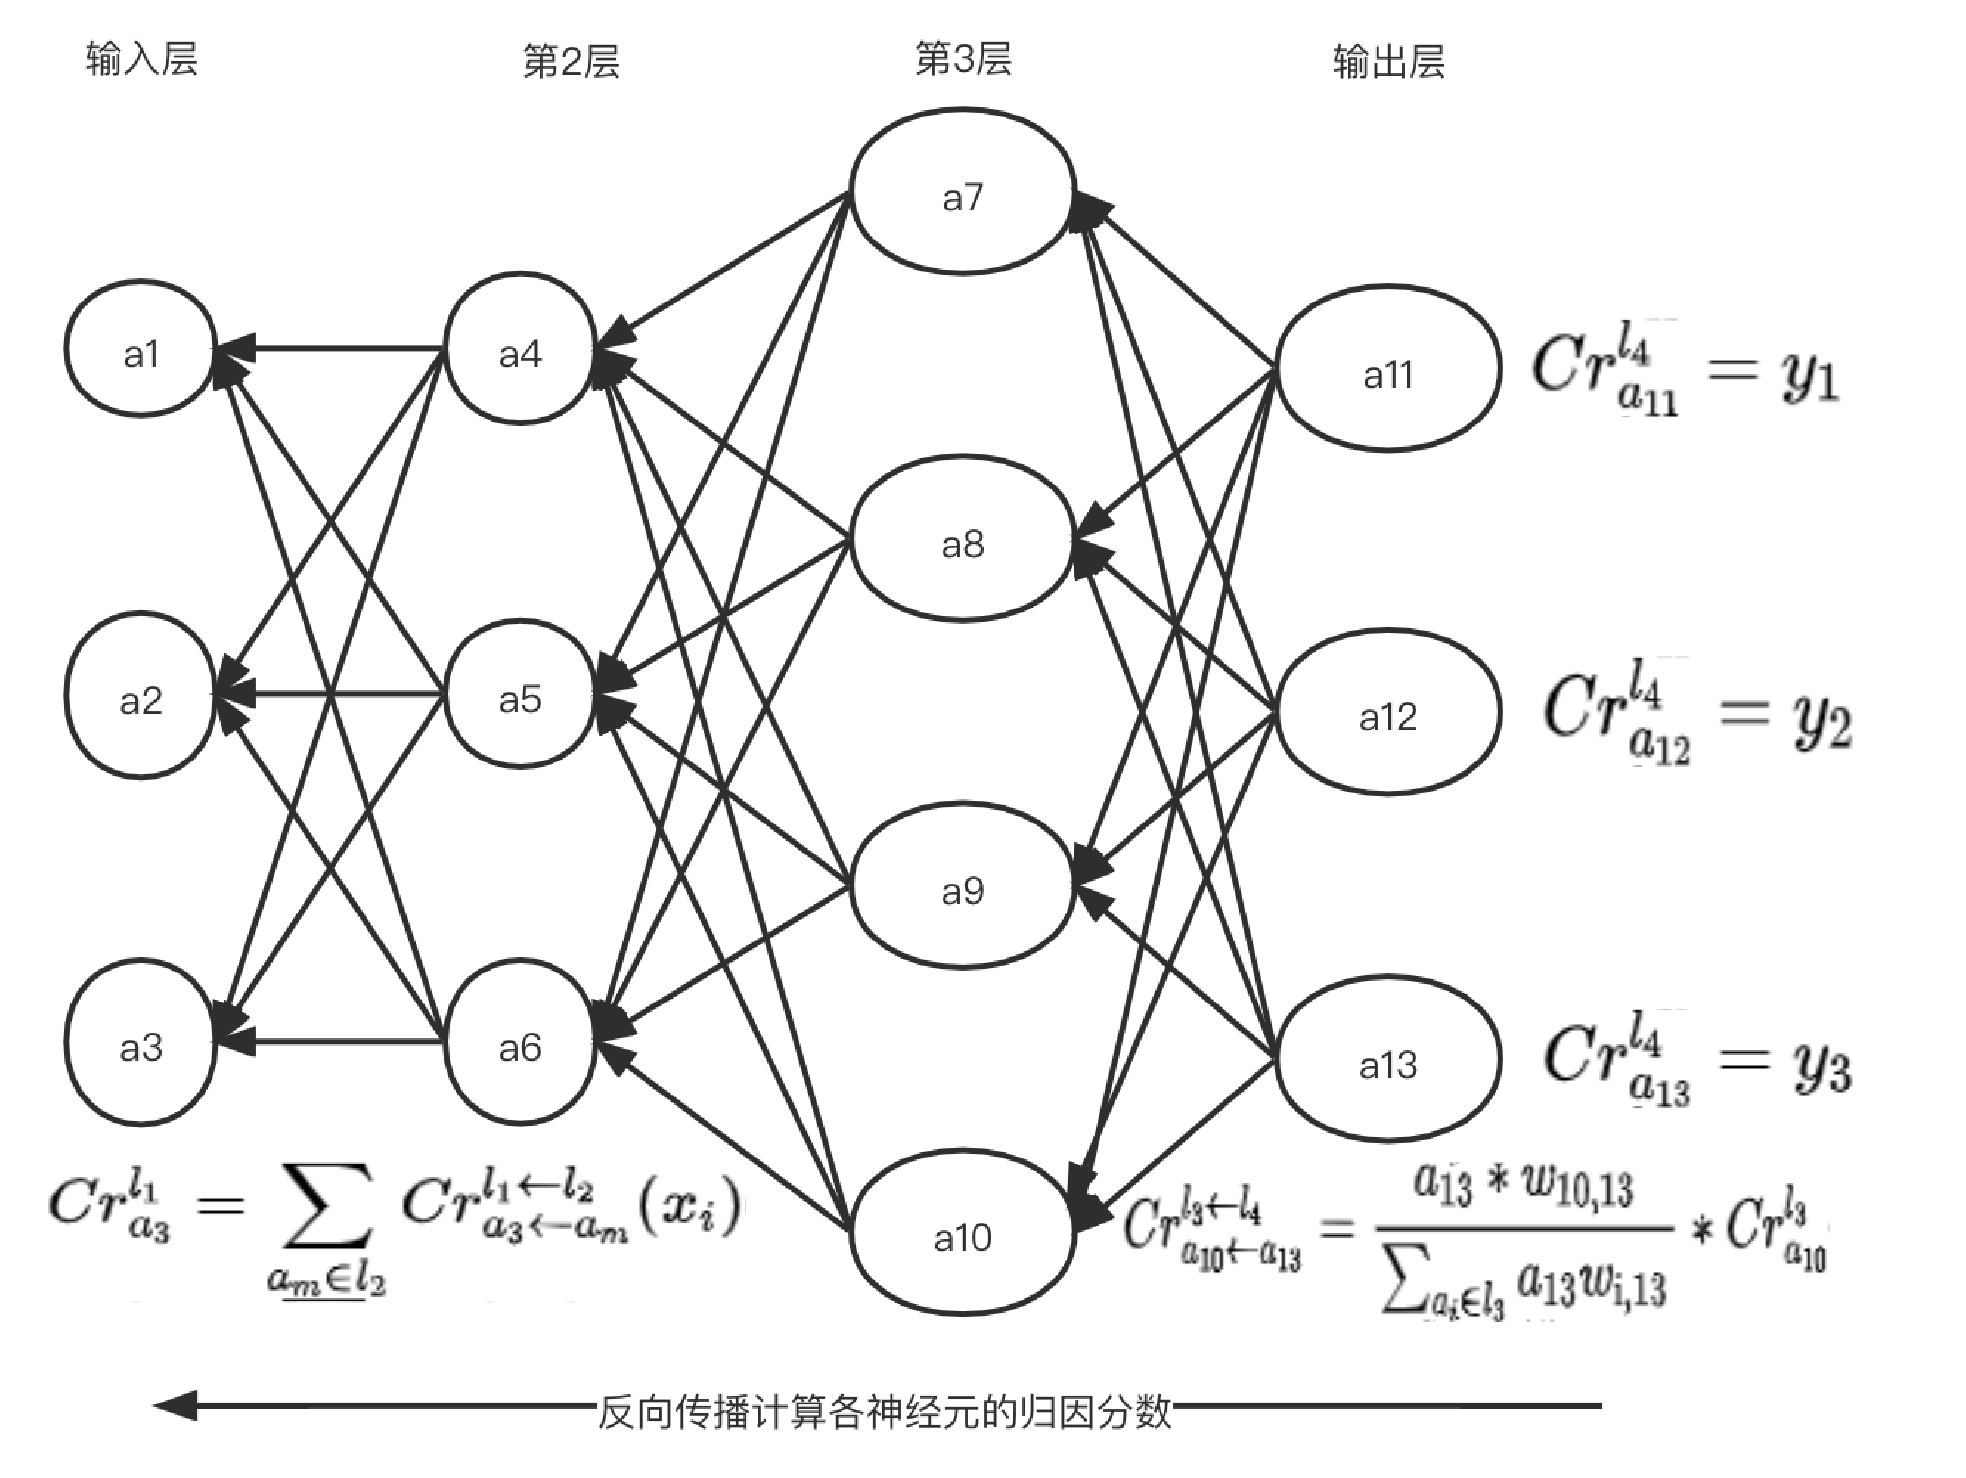
\includegraphics[scale=0.3]{fig2/C3/自适应-反向传播}%联邦学习的系统架构
	\caption{逐层关联传播算法:根据反向传播计算各神经元的归因分数}
	\label{fig:逐层关联传播算法:根据反向传播计算各神经元的归因分数}	
\end{figure}

% 第m-1层的神经元$a_{i}$对于第m层的神经元的归因分数$Cr_{a_{i} \leftarrow a_{j}}^{l_{m-1} \leftarrow l_{m}}\left(x_{i}\right)$等于:
% \begin{equation}
% Cr_{a_{i} \leftarrow a_{j}}^{l_{m-1} \leftarrow l_{m}}\left(x_{i}\right)={\sum_{j=1}^{n} R_{a_{i} \leftarrow a_{j}}^{(l_{m-1},l_{m})}},a_{j} \in l_{m}
% % Cr_{a_{i} \leftarrow a_{j}}^{l_{m-1} \leftarrow l_{m}}\left(x_{i}\right)=\left\{\begin{array}{cc}\frac{a_{i} w_{i, j}}{\sum_{a_{i} \in l_{m-1} a_{i} w_{i, j}}} Cr_{a_{j}}^{l_{m}}\left(x_{i}\right) & \sum_{a_{i} \in l_{m-1}} a_{i} w_{i, j} \neq 0 \\ \mu & \sum_{a_{i} \in l_{m-1}} a_{i} w_{i, j}=0\end{array}\right.
% \end{equation}

如图\ref{fig:逐层关联传播算法:根据反向传播计算各神经元的归因分数}所示,第1层的神经元$a_{3}$的归因分数表示为:
$$
C r_{a_{3}}^{l_{1}}=\sum_{a_{m} \in l_{2}} Cr_{a_{3} \leftarrow a_{m}}^{l_{1} \leftarrow l_{2}}\left(x_{i}\right)
$$

根据以上公式的推导,我们能得到神经网络中各个神经元的归因分数。那么模型的输出可以表示为各层神经元归因分数的累加和:
$$
\begin{aligned}
\sum f\left(x_{i}, \omega_{i}^{r}\right) &=Cr_{a_{11}}^{l_{4}}\left(x_{i}\right)+Cr_{a_{12}}^{l_{4}}\left(x_{i}\right)+Cr_{a_{13}}^{l_{4}}\left(x_{i}\right)\\
&+Cr_{a_{7}}^{l_{3}}\left(x_{i}\right)+Cr_{a_{8}}^{l_{3}}\left(x_{i}\right)+Cr_{a_{9}}^{l_{3}}\left(x_{i}\right)+Cr_{a_{10}}^{l_{3}}\left(x_{i}\right)\\
&+Cr_{a_{4}}^{l_{2}}\left(x_{i}\right)+Cr_{a_{5}}^{l_{2}}\left(x_{i}\right)+Cr_{a_{6}}^{l_{2}}\left(x_{i}\right)\\
&+Cr_{a_{1}}^{l_{1}}\left(x_{i}\right)+Cr_{a_{2}}^{l_{1}}\left(x_{i}\right)+Cr_{a_{3}}^{l_{1}}\left(x_{i}\right)
\end{aligned}
$$

其中,$\sum f\left(x_{i}, \omega_{i}^{r}\right)$等于模型的总输出。根据以上公式,已经可以得到每个神经元的归因分数和神经网络各层的归因分数。

根据每个神经元的归因分数和模型输出,我们可以计算出每层神经网络对模型输出的平均贡献:
\begin{equation}\label{eq:属性添加自适应扰动}
Cr_{j}\left(x_{i}\right)=\frac{1}{n} \sum_{i=1}^{n} Cr_{x_{i, j}}\left(x_{i}\right), j \in[1, u]
% Cr_{j}\left(x_{i}\right)=\frac{Cr_{a_{i}}^{l_{m}}\left(x_{i}\right)}{\sum_{i=1}^{n} Cr_{x_{i, j}}\left(x_{i}\right)}, j \in[1, u]
\end{equation}

和每个神经元$a_{i}$对于模型输出的贡献率:
\begin{equation}\label{eq:属性添加自适应扰动}
\ddot{Cr_{j}}\left(x_{i}\right)=\frac{Cr_{a_{i}}^{l_{m}}\left(x_{i}\right)}{\sum_{i=1}^{n} Cr_{x_{i, j}}\left(x_{i}\right)}, j \in[1, u]
\end{equation}

\subsubsection{梯度的自适应加躁}
% 然后,我们引入了两个调整参数$C$和$p$。其中,$C$代表贡献率阈值,用于决定梯度对模型结果输出的归因分数是高还是低,其值由联邦学习中的本地用户自己定义,即贡献超过阈值$C$的梯度对输出的贡献更大,我们向所有这些梯度注入自适应高斯噪声。当归因分数低于阈值$C$时,对这些梯度进行概率选择。也就是说,我们抛弃概率为$1-p$的原始数据,并对一些概率为$p$的梯度注入自适应高斯噪声。该公式如下:
% \begin{equation}\label{eq:神经网络加噪}
% \tilde{x}_{i, j}=\left\{\begin{array}{ll}
% \ddot{x}_{i, j} & \alpha \geq C \\
% \bar{x}_{i, j} & \alpha<C
% \end{array}\right.
% \end{equation}

% 其中$\alpha$代表该层神经元的贡献率:$\alpha=\frac{\left|\ddot{Cr}_{j}\right|}{\sum_{j=1}^{u}\left|\ddot{Cr}_{j}\right|}$,根据贡献率阈值C将神经层分为两类。当$\alpha>C$时,根据贡献率对所有梯度添加对应的高斯噪声;当$\alpha<C$时,对属性进行概率选择:
% \begin{equation}\label{eq:神经网络加噪2}
% \bar{x}_{i, j}=\left\{\begin{array}{l}
% \ddot{x}_{i, j} \text { with probability } p \\
% x_{i, j} \text { with probability } 1-p
% \end{array}\right.
% \end{equation}

所谓梯度的自适应加躁,即根据神经元对模型输出的贡献率分配不同的隐私预算。对于贡献率较大的的特征,分配的隐私预算更高,即在梯度上添加的噪声量更小;反之亦然。在上一节中,通过逐层关联传播算法对模型进行预训练,得到了每层神经元对于模型输出结果的贡献率,贡献率决定了给梯度加躁的隐私预算的大小。

在完成模型的预训练之后,进入模型的正式训练环节。重新初始化神经网络的训练参数,根据第二章所介绍的随机梯度下降算法,找到最终的权重参数$\widehat{\boldsymbol{\theta}} \in \mathbb{R}^{d}$ ,使经验风险值最小。具体的算法如\ref{梯度的自适应加躁算法}所示,关键的步骤包括:计算损失函数对于所有权重和偏置的梯度,分配相应的隐私预算,在梯度上添加高斯噪声,最后进行梯度下降,重复上述步骤直至模型收敛,最后输出权重$\theta_{t}$。\\。

\begin{algorithm}[!htb]
	\caption{梯度的自适应加躁算法}
	\label{梯度的自适应加躁算法}
	\begin{algorithmic}[1]
		\footnotesize
		\STATE \textbf{输入:} 数据集 $\left\{x_{1}, \ldots, x_{N}\right\}$,损失函数$\mathcal{L}(\theta)=$ $\frac{1}{N} \sum_{i} \mathcal{L}\left(\theta, x_{i}\right)$,学习率$\eta_{t}$, 初始隐私预算$\sigma_{l}$, 批大小$L$
		\STATE 初始化:模型权重$\theta_{0}$
		\FOR{ $t \in[T]$}
			\STATE 以概率$L / N$随机采样一批数据集$L_{t}$
			\FOR{$x_{i} \in L_{t}$ }
				\STATE 计算梯度:$\mathbf{g}_{t}\left(x_{i}\right) \leftarrow \nabla_{\theta_{t}} \mathcal{L}\left(\theta_{t}, x_{i}\right)$
				\STATE 根据神经元对模型输出的贡献率分配相应的隐私预算:$\sigma_{i}=\frac{\sigma_{l}}{\ddot{Cr_{j}}\left(x_{i}\right)}$
				\STATE 在梯度上添加高斯噪声:$\tilde{\mathbf{g}}_{t} \leftarrow \frac{1}{L} \sum_{i}\left(\overline{\mathbf{g}}_{t}\left(x_{i}\right)+\mathcal{N}\left(0, S_{f}^{2} \cdot \sigma_{i}^{2}\right)\right)$
			\ENDFOR
			\STATE 计算平均加躁梯度:$\tilde{w}^{t}=\frac{1}{L} \sum_{x_{i} \in L_{t}} \tilde{w}^{t}(x_{i})$
			\STATE 梯度下降:$\theta^{t+1}=\theta^{t}-\eta^{t} \tilde{w}^{t}$
		\ENDFOR
		\STATE \textbf{输出:} $\theta_{t}$
	\end{algorithmic}
\end{algorithm}

\subsection{梯度的自适应裁剪算法}
在传统的差分隐私随机梯度下降算法中,提供隐私保护的常用技术是限制函数的敏感度并添加与敏感度界限成比例的高斯噪声。而且,相关研究表明合适的梯度裁剪能加快模型的收敛速度。为此,我们需要在每一轮SGD上限制梯度的敏感性。Abadi\upcite{ref65}等人提出通过梯度裁剪使得梯度保持在[-C,C]的范围内,以保证函数的敏感度有界。如果损失函数是可微的(如果不可微,则使用子梯度)和Lipschitz有界的,用Lipschitz 界限制梯度范数,并用它来推导出梯度的敏感度。 如果损失函数导数作为输入的函数有界,可以推导出梯度敏感度。如果损失函数不像深度学习应用中那样具有已知的Lipschitz界,则很难推导出梯度范数的先验界。

在固定的梯度裁剪算法中,训练初期无从得知梯度范数的先验界限,所以基本是采用一个固定的梯度范数进行裁剪。假设用户上传的梯度向量为$\tilde{\mathbf{g}}_{t}$,根据固定梯度范数进行裁剪后,梯度缩放为$\mathbf{g} / \max \left(1, \frac{\|\mathbf{g}\|_{2}}{C}\right)$, 其中 $C$是梯度阈值。对于梯度的裁剪能保证梯度值小于梯度阈值时,也就是当$\|\mathbf{g}\|_{2} \leq C$ ,$\mathbf{g}$保持不变;当$\|\mathbf{g}\|_{2}>C$时, 它会按照裁剪比例缩小为 $C$。在每次训练迭代中,可以使用经验值来获得梯度范数的近似界限,并在损失函数近似界限处裁剪梯度。然而,经验值的可用性是一个强有力的假设,在没有经验值的情况下如何针对自适应添加的噪声裁剪梯度是一个难题。如果梯度阈值$C$ 的值太小,那么裁剪后的梯度会较小,算法添加的噪声较小时可能会破坏梯度估计的无偏性;另一方面,如果不对梯度进行裁剪,大量的噪声添加到每个梯度会导致模型的可用性大大降低。神经网络的架构、损失函数本身、数据的缩放都会影响裁剪范数的选择。本章节所设计的方案根据训练轮数和梯度变化的偏差与方差动态的更新梯度裁剪阈值,对梯度进行自适应裁剪。

% 假设在随机梯度下降算法的第$t$轮迭代过程中,梯度向量表示为$g^{t}=\left(g_{1}^{t}, g_{2}^{t}, . ., g_{d}^{t}\right)$。根据差分隐私的定义,除了第一个维度之外,不需要向其他维度添加太多噪声。这促使我们自适应地将不同的噪声水平添加到不同的维度,以最小化添加噪声后梯度的 $\ell_{2}$-范数。我们提出了两个额外的辅助向量 $a^{t}=\left(a_{1}^{t}, a_{2}^{t}, . ., a_{d}^{t}\right)$和$b^{t}=\left(b_{1}^{t}, b_{2}^{t}, . ., b_{d}^{t}\right)$,初始值为$a^{t}=(0,0, \ldots, 0)$,$b^{t}=(1, 1, \ldots 1)$。

在深度学习的模型训练中,模型的泛化能力取决于预测值的方差、偏差和数据的噪声。偏差度量的是模型预测值与真实值之间的偏离程度;方差度量的是训练数据的变动给模型预测结果带来的影响,也就是噪声的添加会影响梯度的方差,而随机梯度的方差决定了SGD算法的收敛速度,梯度的裁剪会影响偏差。因此我们更关注梯度更新的方差和偏差来决定如何对梯度进行裁剪。之前的梯度裁剪算法给梯度本身添加了额外的噪声,因此我们考虑根据训练时观察到的历史梯度的统计数据来设置梯度阈值,通过计算梯度更新的偏差和方差在每轮随机梯度下降中更新梯度阈值。

首先,我们对梯度进行裁剪,裁剪后的梯度为$\hat{w}^{t}$:
\begin{equation}
\hat{w}^{t}=\operatorname{clip}\left(w^{t}, C^{t}\right) \triangleq w^{t} \cdot \min \left(1, \frac{C^{t}}{\left\|w^{t}\right\|_{2}}\right)
\end{equation}

然后对保留的梯度$\hat{w}^{t}$根据神经元的归因分数添加高斯噪声 $\mathcal{N}\left(0, S_{f}^{2} \cdot \sigma^{2}\right)$:
\begin{equation}
\tilde{w}^{t}=\hat{w}^{t}+N^{t} \quad N^{t} \sim \mathcal{N}\left(0, \sigma^{2} I\right)
\end{equation}

理想情况下,裁剪后的梯度对于模型的收敛的影响应该很小,因此我们希望在每一轮梯度下降算法中找到最佳的裁剪阈值$C^{t}$使$\mathbb{E}\left\|\tilde{w}^{t}-w^{t}\right\|^{2}$最小。 

根据三角不等式和Jensen不等式,更新前后的梯度方差与偏差可以表示为以下公式:
\begin{equation}\label{eq:梯度更新后的方差与偏差}
\operatorname{bias}\left(\tilde{w}^{t}\right) \leq \operatorname{bias}\left(w^{t}\right)+2 \mathbb{E}\left\|\tilde{w}^{t}-w^{t}\right\| \text {和} \operatorname{Var}\left(\tilde{w}^{t}\right) \leq 3 \operatorname{Var}\left(w^{t}\right)+6 \mathbb{E}\left\|\tilde{w}^{t}-w^{t}\right\|^{2}
\end{equation}

我们通过约束$\mathbb{E}\left\|\tilde{w}^{t}-w^{t}\right\|$找到最佳的裁剪阈值$C^{t}$,将上述公式转换为:
\begin{equation}\label{eq:梯度更新后的方差与偏差2}
\mathbb{E}\left\|\tilde{w}^{t}-w^{t}\right\|^{2}=\left\|w^{t}\right\|^{2}\left(1-\frac{1}{\max \left(1,\left\|w^{t}\right\|\right)}\right)^{2}+{C^{t}}^{2} \sigma^{2}
\end{equation}

公式\ref{eq:梯度更新后的方差与偏差2}中的第一项对应于变换后的梯度$w_{t}$可能被裁剪的情况,第二项对应于注入到裁剪梯度中的高斯噪声。理想情况下,我们希望能找到使上述表达式\ref{eq:梯度更新后的方差与偏差2}最小化的裁剪阈值$C^{t}$。

为了使预测的梯度值的偏差最小,根据上一轮迭代得到的加躁梯度,通过指数渐进平均估计可得:
\begin{equation}\label{eq:梯度偏差估计}
m^{t}=\beta_{1} m^{t-1}+\left(1-\beta_{1}\right) \tilde{w}^{t}
\end{equation}
其中$\beta_{1}$是指数移动平均线的衰减参数。

为了使预测的梯度值的方差最小, 假使梯度没有被裁剪时,根据$\tilde{w}^{t}=w^{t}+C^{t} N^{t}$,从$\mathbb{E}\left(\tilde{w}_{i}^{t}-m_{i}^{t}\right)^{2}$推导出$\mathbb{E}\left(w_{i}^{t}-m_{i}^{t}\right)^{2}$:
$$
\begin{aligned}
\mathbb{E}\left(w_{i}^{t}-m_{i}^{t}\right)^{2} &=\mathbb{E}\left(\tilde{w}_{i}^{t}-m_{i}^{t}\right)^{2}+\mathbb{E}\left(C^{t} N_{i}^{t}\right)^{2}+2 \mathbb{E}\left(-C^{t} N_{i}^{t}\right)\left(w_{i}^{t}+C^{t} N_{i}^{t}-m_{i}^{t}\right) \\
&=\mathbb{E}\left(\tilde{w}_{i}^{t}-m_{i}^{t}\right)^{2}-\mathbb{E}\left(C^{t} N_{i}^{t}\right)^{2}-2 \mathbb{E}\left(C^{t} N_{i}^{t}\right)\left(w_{i}^{t}-m_{i}^{t}\right) \\
&=\mathbb{E}\left(\tilde{w}_{i}^{t}-m_{i}^{t}\right)^{2}-{C^{t}}^{2} \sigma^{2}
\end{aligned}
$$
我们需要确保$\left(w_{i}^{t}-m_{i}^{t}\right)^{2}$满足上限和下限:
$$
\left(w_{i}^{t}-m_{i}^{t}\right)^{2} \approx \min \left(\max \left(\left(\tilde{w}_{i}^{t}-m_{i}^{t}\right)^{2}-{C^{t}}^{2} \sigma^{2}, h_{1}\right), h_{2}\right)
$$
其中,$h_{1}$和$h_{2}$为常数,我们使用上式的指数移动平均值来估计方差:
\begin{equation}\label{eq:梯度方差估计}
\begin{aligned}
v_{t} &=\min \left(\max \left(\left(\tilde{g}_{i}^{t}-m_{i}^{t}\right)^{2}-{C^{t}}^{2} \sigma^{2}, h_{1}\right), h_{2}\right) \\
\left(s_{i}^{t}\right)^{2} &=\beta_{2}\left(s_{i}^{t-1}\right)^{2}+\left(1-\beta_{2}\right) v_{t}
\end{aligned}
\end{equation}

梯度自适应裁剪算法在每个训练迭代时刻t设置梯度裁剪阈值$C^{t}$,其中每个迭代对应于一个minibatch的处理,接着跟踪训练过程中看到的每个批次的梯度范数。在每一轮的梯度聚合之后,根据公式\ref{eq:梯度偏差估计}和\ref{eq:梯度方差估计}计算梯度变化的方差和偏差,更新梯度裁剪阈值$C^{t}$使$\mathbb{E}\left\|\tilde{w}^{t}-w^{t}\right\|^{2}$最小。将自适应梯度裁剪应用到随机梯度下降算法中,具体算法如\ref{梯度的自适应裁剪算法}所示。梯度自适应裁剪算法的动态性导致了$C^{t}$的自适应设置,该设置由数据、网络和损失动态决定,而不是由用户在训练初始阶段设置固定的裁剪值,根据神经网络各层的均值和统计特征进行梯度裁剪既能限制敏感度有界,也能保留有效的梯度信息。

\begin{algorithm}[!htb]
	\caption{梯度的自适应裁剪算法}
	\label{梯度的自适应裁剪算法}
	\begin{algorithmic}[1]
		\footnotesize
		\STATE \textbf{输入:} 数据集 $\left\{x_{1}, \ldots, x_{N}\right\}$,损失函数$\mathcal{L}(\theta)=$ $\frac{1}{N} \sum_{i} \mathcal{L}\left(\theta, x_{i}\right)$,学习率$\eta_{t}$,隐私预算$\sigma$,批大小$L$,裁剪阈值$C^{0}$
		\STATE 初始化:模型权重$\theta_{0}$
		\FOR{ $t \in[T]$}
			\STATE 以概率$L / N$随机采样一批数据集$L_{t}$
			\FOR{$x_{i} \in L_{t}$ }
				\STATE 计算梯度:$\mathbf{w}_{t}\left(x_{i}\right) \leftarrow \nabla_{\theta_{t}} \mathcal{L}\left(\theta_{t}, x_{i}\right)$
				\STATE 梯度裁剪:$\hat{w}^{t}=\operatorname{clip}\left(w^{t}, C^{t}\right) \triangleq w^{t} \cdot \min \left(1, \frac{C^{t}}{\left\|w^{t}\right\|_{2}}\right)$
				\STATE 在梯度上添加高斯噪声:$\tilde{w}^{t}\leftarrow \left(\hat{w}^{t}\left(x_{i}\right)+\mathcal{N}\left(0, S_{f}^{2} \cdot \sigma^{2}\right)\right)$
			\ENDFOR
			\STATE 计算平均加躁梯度:$\tilde{w}^{t}=\frac{1}{L} \sum_{x_{i} \in L_{t}} \tilde{w}^{t}(x_{i})$
			\STATE 梯度下降:$\theta_{t+1} \leftarrow \theta_{t}-\eta_{t} \tilde{w}^{t}$
			\STATE 根据公式\ref{eq:梯度方差估计}和\ref{eq:梯度偏差估计}计算梯度变化的方差和偏差,更新$C^{t}$
		\ENDFOR
		\STATE \textbf{输出:} $\theta_{t}$
	\end{algorithmic}
\end{algorithm}

\subsection{基于自适应差分隐私的SGD算法}

结合前两节所提出的自适应梯度加躁和裁剪算法,我们设计了算法\ref{基于自适应差分隐私的随机梯度下降算法}。在本地客户端训练过程中,在随机梯度下降算法中并使用自适应梯度裁剪算法动态调整梯度阈值,添加自适应噪声使算法整体满足$(\epsilon, \delta)$-差分隐私,最小化目标函数$f(\theta)=\frac{1}{N} \sum_{k=1}^{N} f_{k}(\theta)$。首先,通过逐层传播算法对模型进行预训练,得到网络中各个神经元的归因分数及其对于模型输出的贡献率。然后运行随机梯度下降算法每一轮用户随机采样小批次的$L$个样本,对于样本集中的每条数据记录,计算损失函数对于所有神经元的权重和偏置的梯度$\mathbf{g}_{t}\left(x_{i}\right)$,然后将梯度裁剪到一个固定的范围[-$C_{t}$,$C_{t}$],从而控制个体数据对输出结果的影响,此时梯度的敏感度为$\Delta_{2}(f)=\max _{x_{i} \in D}\left\|\hat{g}^{t}\right\|_{2} \leq C$。完成梯度裁剪后,对梯度添加与贡献率成反比的高斯噪声,得到满足$(\epsilon, \delta)$-差分隐私的梯度数据。之后计算批次大小为$L$的样本集的平均加躁梯度,然后进行梯度下降,计算梯度更新的方差和偏差,调整梯度裁剪阈值$C^{t}$。不断的重新采样数据,迭代地进行梯度下降的训练,使目标函数最小,输出模型权重$\theta_{t}$。
\begin{algorithm}[!htb]
	\caption{基于自适应差分隐私的随机梯度下降算法}
	\label{基于自适应差分隐私的随机梯度下降算法}
	\begin{algorithmic}[1]
		\footnotesize
		\STATE \textbf{输入:} 目标函数$f(\theta)=\frac{1}{N} \sum_{k=1}^{N} f_{k}(\theta)$,学习率$\eta^{t}$,训练批次大小$L$,高斯噪声参数$\sigma_{l}$,裁剪阈值$C^{0}$
		\STATE 初始化:$m^{0}=0 \cdot 1, s^{0}=\sqrt{h_{1} h_{2}} \cdot 1$
		\STATE 随机初始化模型参数:$\theta^{0}$
		\FOR{ $t \in[T]$}
			\STATE 以概率$L / N$随机采样一批数据集$L_{t}$
			\FOR{$x_{i} \in L_{t}$}
				\STATE 根据逐层传播算法计算神经元对于模型输出的归因分数:$Cr_{a_{i}}^{l_{m}}\left(x_{i}\right)=\sum_{a_{j} \in l_{m+1}} Cr_{a_{i} \leftarrow a_{j}}^{l_{m} \leftarrow l_{m+1}}\left(x_{i}\right)$
				\STATE 计算神经元对模型输出的贡献率:$\ddot{Cr_{j}}\left(x_{i}\right)=\frac{Cr_{a_{i}}^{l_{m}}\left(x_{i}\right)}{\sum_{i=1}^{n} Cr_{x_{i, j}}\left(x_{i}\right)}, j \in[1, u]$
				\STATE 计算梯度:$\mathbf{g}_{t}\left(x_{i}\right) \leftarrow \nabla_{\theta_{t}} \mathcal{L}\left(\theta_{t}, x_{i}\right)$
				\STATE 梯度裁剪:$\hat{g}^{t}=\operatorname{clip}\left(g^{t}, C^{t}\right) \triangleq g^{t} \cdot \min \left(1, \frac{C^{t}}{\left\|g^{t}\right\|_{2}}\right)$
				\STATE 根据贡献率分配相应的隐私预算:$\sigma_{i}=\frac{\sigma_{l}}{\ddot{Cr_{j}}\left(x_{i}\right)}$
				\STATE 在梯度上添加高斯噪声:$\tilde{g}^{t}\leftarrow \left(\hat{g}^{t}\left(x_{i}\right)+\mathcal{N}\left(0, S_{f}^{2} \cdot {\sigma_{i}}^{2}\right)\right)$
			\ENDFOR
			\STATE 计算平均加躁梯度:$\tilde{g}^{t}=\frac{1}{L} \sum_{x_{i} \in L_{t}} \tilde{g}^{t}(x_{i})$
			\STATE 梯度下降:$\theta^{t+1}=\theta^{t}-\eta^{t} \tilde{g}^{t}$
			\STATE 根据公式\ref{eq:梯度方差估计}和\ref{eq:梯度偏差估计}计算梯度变化的方差和偏差,更新$C^{t}$
		\ENDFOR
		\STATE \textbf{输出:} $\theta_{t}$
	\end{algorithmic}
\end{algorithm}

当噪声参数满足$\frac{\sigma_{l}}{C^{0}}=\frac{\sqrt{2 \ln (1.25 / \delta)}}{\epsilon}$时,添加噪声后的梯度满足$(\epsilon, \delta)$-差分隐私。根据差分隐私的可组合性与后处理不变性,添加噪声后的数据满足差分隐私,该性质会传递到后续的处理过程,最终得到的模型权重也满足$(\epsilon, \delta)$-差分隐私。

在下一节,我们将给出自适应差分隐私SGD算法的整体隐私预算$(\epsilon, \delta)$分析。

\section{隐私参数分析}

% 自适应差分隐私SGD算法在梯度下降过程中根据神经元对于模型输出的贡献率在梯度上添加高斯噪声,算法整体满足$(\epsilon, \delta)$-差分隐私。证明如下:

% \begin{proof}
% 假设现有相邻数据集$D$和$D^{\prime}$,两个数据集上的第n条数据记录$x_{n}$和$x_{n}^{\prime}$不同,在模型上的输出分别为$F_{\theta}$和$F_{\theta}^{\prime}$,$C(D)$和$C(D^{\prime})$分别代表这两个数据集的总归因分数:

% \begin{equation}
% Cr(D)=\left\{Cr_{j}\left(x_{i}\right)\right\}, j \in[1, u], \text {其中} Cr_{j}\left(x_{i}\right)=\frac{1}{n} \sum_{i=1}^{n} Cr_{x_{i, j}}\left(x_{i}\right), j \in[1, u]
% \end{equation}

% \begin{equation}
% Cr\left(D^{\prime}\right)=\left\{Cr_{j}\left(x_{i}^{\prime}\right)\right\}, j \in[1, u], \text {其中} Cr_{j}\left(x_{i}^{\prime}\right)=\frac{1}{n} \sum_{i=1}^{n} Cr_{x_{i, j}^{\prime}}\left(x_{i}^{\prime}\right), j \in[1, u]
% \end{equation}

% 根据神经元的归因分数在其梯度$\mathbf{g}_{t}\left(x_{i}\right) \leftarrow \nabla_{\theta_{t}} \mathcal{L}\left(\theta_{t}, x_{i}\right)$上添加自适应的噪声:
% \begin{equation}\label{eq:神经网络加噪3}
% \tilde{\mathbf{g}}_{t} \leftarrow \frac{1}{L} \sum_{i}\left(\overline{\mathbf{g}}_{t}\left(x_{i}\right)+\mathcal{N}\left(0, S_{f}^{2} \cdot \sigma^{2}\right)\right)
% \end{equation}

% 其中隐私预算与贡献率成正比:$\sigma_{i}=\ddot{Cr_{j}}\left(x_{i}\right) * \sigma_{l}$。

% 首先,通过敏感度公式计算梯度的$L_{2}$敏感度:
% \begin{equation}\label{eq:贡献敏感度}
% \begin{aligned}
% \Delta_{2}(f)=\max _{x_{i} \in D}\left\|\nabla_{\theta} \operatorname{loss}\left(x_{i}, \theta\right)\right\|_{2} \leq C
% % S_{f} &=\frac{1}{|D|} \sum_{j=1}^{u}\left\|\sum_{x_{i} \in D} Cr_{x_{i, j}}\left(x_{i}\right)-\sum_{x_{i}^{\prime} \in D^{\prime}} Cr_{x_{i, j}^{\prime}}\left(x_{i}^{\prime}\right)\right\|_{2} \\ &=\frac{1}{|D|} \sum_{j=1}^{u}\left\|Cr_{x_{n, j}}\left(x_{n}\right)-Cr_{x_{n, j}^{\prime}}\left(x_{n}^{\prime}\right)\right\|_{2} \\ & \leq \frac{2}{|D|} \max \sum_{j=1}^{u}\left\|C_{x_{i, j}}\left(x_{i}\right)\right\|_{2} \\ & \leq \frac{2 u}{|D|} 
% \end{aligned}
% \end{equation}

% 当噪声参数满足$\frac{\sigma}{C}=\frac{\sqrt{2 \ln (1.25 / \delta)}}{\epsilon}$时,添加噪声后的梯度满足$(\epsilon, \delta)$-差分隐私。根据差分隐私的可组合性与后处理不变性,添加噪声后的数据满足差分隐私,该性质会传递到后续的处理过程,最终得到的模型权重也满足$(\epsilon, \delta)$-差分隐私。

% 对于高斯机制的证明,因为高斯机制实现的是松弛差分隐私,将模型的输出分为两部分,证明其中一部分严格满足差分隐私,另一部分违反差分隐私。因此,我们将输出分为两部分,证明第一部分$S_{1}$被$\epsilon$约束,第二部分$S_{2}$小于$\delta$:
% \begin{equation}
% \begin{aligned}
% \operatorname{Pr}_{x_{i} \sim \mathcal{N}\left(0, S_{f}^{2} \cdot \sigma^{2}\right)}[f(x)+x \in S]=& \operatorname{Pr}_{x \sim \mathcal{N}\left(0, S_{f}^{2} \cdot \sigma^{2}\right)}\left[f(x)+x \in S_{1}\right] \\ &+\operatorname{Pr}_{x \sim \mathcal{N}\left(0, S_{f}^{2} \cdot \sigma^{2}\right)}\left[f(x)+x \in S_{2}\right] \\ \leq & \operatorname{Pr}_{x \sim \mathcal{N}\left(0, S_{f}^{2} \cdot \sigma^{2}\right)\right)}\left[f(x)+x \in S_{1}\right]+\delta \\ \leq & e^{\varepsilon}\left(\operatorname{Pr}_{x \sim \mathcal{N}\left(0, S_{f}^{2} \cdot \sigma^{2}\right)}\left[f(y)+x \in S_{1}\right]\right)+\delta 
% \end{aligned}
% \end{equation}

% 其中,$u$和$|D|$分别表示神经网络中神经元和神经层的数量,然后可以得到:
% \begin{equation}\label{贡献数量和元组}
% \begin{aligned}
% \frac{\operatorname{Pr}(\ddot{Cr}(D))}{\operatorname{Pr}\left(\ddot{Cr}\left(D^{\prime}\right)\right)} &=\frac{\prod_{j=1}^{u} \exp \left(\frac{\epsilon_{c}\left\|\frac{1}{|D|} \sum_{x_{i} \in D} Cr_{j}\left(x_{i}\right)-\ddot{Cr}_{j}\left(x_{i}\right)\right\|_{2}}{S_{f}}\right)}{\prod_{j=1}^{u} \exp \left(\frac{\epsilon_{c}\left\|\frac{1}{\left|D^{\prime}\right|} \sum_{x_{i}^{\prime} \in D^{\prime}} Cr_{j}\left(x_{i}^{\prime}\right)-\ddot{Cr}_{j}\left(x_{i}^{\prime}\right)\right\|_{2}}{S_{f}}\right)} \\
% &=\prod_{j=1}^{u} \exp \left(\frac{\epsilon_{c}}{|D| S_{f}}\left\|Cr_{j}\left(x_{n}\right)-Cr_{j}\left(x_{n}^{\prime}\right)\right\|_{2}\right) \\
% & \leq \prod_{j=1}^{u} \exp \left(\frac{\epsilon_{c}}{|D| S_{f}} \max \left\|Cr_{j}\left(x_{n}\right)\right\|_{2}\right) \\
% &=\exp \left(\epsilon_{c} \frac{\max _{x_{i} \in D} \sum_{j=1}^{u}\left\|Cr_{j}\left(x_{n}\right)\right\|_{2}}{|D| S_{f}}\right) \\
% & \leq \exp \left(\epsilon_{c}\right)
% \end{aligned}
% \end{equation}

% 因此,根据梯度归因分数添加高斯噪声的算法是满足$\epsilon_{c}$-差分隐私的。
% \end{proof}
% 接着我们根据归因分数对于梯度进行概率选择添加噪声,我们接下来证明这部分的算法是满足$\epsilon_{l}$-差分隐私的。

% 假设两个相邻的数据集$D_{i}^{t}$和$D_{i}^{t^{\prime}}$,其中数据记录$x_{n}$和$x_{n}^{\prime}$不同,$z\left(D_{i}^{t}\right)$和$z\left(D_{i}^{t^{\prime}}\right)$分别为两个数据集上训练采用的线性变换函数。

% 一般来说,我们把偏置项视为第一类数据属性,即:$x_{i,0}=b_{i}$。线性转换可以改写为:$\ddot{\mathbf{z}}_{x \in D_{i}^{t}}(\omega)=\ddot{\mathbf{x}} * \omega$。线性变换函数的敏感度$S_{f}$为:
% \begin{equation}
% \begin{aligned}
% S_{f} &=\sum_{a_{i} \in l_{1}} \sum_{j=1}^{u}\left\|\sum_{x_{i} \in D_{i}^{t}} x_{i, j}-\sum_{x_{i}^{\prime} \in D_{i}^{t^{\prime}}} x_{i, j}^{\prime}\right\|_{1} \\
% &=\sum_{a_{i} \in l_{1}} \sum_{j=1}^{u}\left\|x_{n, j}-x_{n, j}^{\prime}\right\|_{1} \\
% & \leq \sum_{a_{i} \in l_{1}} \sum_{j=1}^{u} \max _{x_{i} \in D_{i}^{t}}\left\|x_{n, j}\right\|_{1} \\
% & \leq \sum_{a_{i} \in l_{1}} u
% \end{aligned}
% \end{equation}

% 其中,$a_{i} \in l_{1}$是指第一个隐藏层$l_{1}$中的神经元$a_{i}$,$u$是数据元组$x_{i} \in D_{i}^{t}$中的属性数。自适应加躁算法包括两个超参数:$C$和$p$,这两个超参数可以适时过滤多余的噪声,再通过超参数调整噪声大小和裁剪阈值后,整体加躁后的梯度的表达式如下:
% \begin{equation}
% \begin{aligned}
% \tilde{x}_{i, j} &=[(1-C)+C * p] * \ddot{x}_{i, j}+C *(1-p) * x_{i, j} \\
% &=[(1-C)+C * p]\left[x_{i, j}+\mathcal{N}\left(0, S_{f}^{2} \cdot \sigma^{2}\right)\right]+[C *(1-p)] x_{i, j} \\
% &=x_{i, j}+[(1-C)+C * p]\left[\mathcal{N}\left(0, S_{f}^{2} \cdot \sigma^{2}\right)\right]
% \end{aligned}
% \end{equation}
% 然后我们可以得到:

% \begin{equation}
% \begin{aligned}
% \frac{\operatorname{Pr}\left(\ddot{\mathbf{z}}_{D_{i}^{t}}(\omega)\right)}{\operatorname{Pr}\left(\ddot{\mathbf{z}}_{D_{i}^{t}}(\omega)\right)} &=\frac{\prod_{a_{i} \in l_{1}} \prod_{j=1}^{u} \exp \left(\frac{\epsilon_{j}\left\|\sum_{x_{i} \in D_{i}^{t}} x_{i, j}-\sum_{x_{i} \in D_{i}^{t}} \tilde{x}_{i, j}\right\|_{1}}{G S_{l}}\right)}{\prod_{a_{i} \in l_{1}} \prod_{j=1}^{u} \exp \left(\frac{\epsilon_{j}\left\|\sum_{x_{i}^{\prime} \in D_{i}^{t^{\prime}}} x_{i, j}^{\prime}-\sum_{x_{i}^{\prime} \in D_{i}^{t^{\prime}}} \tilde{x}_{i, j}^{\prime}\right\|_{1}}{G S_{l}}\right)} \\
% & \leq \prod_{a_{i} \in l_{1}} \prod_{j=0}^{u} \exp \left(\frac{\epsilon_{j}}{G S_{l}}\left\|\sum_{x_{i} \in D_{i}^{t}} x_{i, j}-\sum_{x_{i}^{\prime} \in D_{i}^{t^{\prime}}} x_{i, j}^{\prime}\right\|_{1}\right) \\
% & \leq \prod_{a_{i} \in l_{1}} \prod_{j=0}^{u} \exp \left(\frac{\epsilon_{j}}{G S_{l}} \max _{x_{i} \in D_{i}^{t}}\left\|x_{n, j}\right\|_{1}\right) \\
% & \leq \exp \left(\epsilon_{l} \frac{\sum_{a_{i} \in l_{1}} u\left[\sum_{j=1}^{u} \frac{\left|\ddot{C}_{j}\right|}{\sum_{j=1}^{u}\left|\ddot{C}_{j}\right|}\right]}{G S_{l}}\right) \\
% &=\exp \left(\epsilon_{l}\right)
% \end{aligned}
% \end{equation}
本章所提出的自适应差分隐私保护方案是通过在随机梯度下降算法上添加自适应的高斯噪声,保护数据的隐私性。在上一节我们已经证明了此算法满足$(\epsilon, \delta)$-差分隐私,那另外一个非常重要的问题就是评估在训练过程中添加噪声所累积的隐私成本。

我们向梯度中添加高斯噪声以得到加躁后的数据,根据第二章所给出的高斯机制的定理可知,当隐私参数$\sigma=\sqrt{2 \log \frac{1.25}{\delta}} / \varepsilon$时,每一批次的输出都满足$(\varepsilon, \delta)$-差分隐私。考虑到每一批次的训练样本是以概率$q=L / N$从数据集中随机采样的,根据隐私放大定理和差分隐私的强组合定理,隐私性由$(\varepsilon, \delta)$-差分隐私扩大到 $(q \varepsilon, q \delta)$-差分隐私。

然而,组合定理并没有考虑到特定的噪声分布,给出的隐私边界较为松散。在本节中,我们采用“Moments Accountant”(MA)机制,去计算算法迭代过程中添加噪声所累积的隐私成本。MA机制计算隐私成本的思想是将隐私损失视为一个随机变量,通过跟踪隐私损失随时间变化的情况,根据组合定理,计算各轮隐私损失的加和分布得到总隐私损失。

假使算法$\mathcal{M}$是满足 $(\epsilon, \delta)$-差分隐私的,那么$\mathcal{M}$中的隐私损失随机变量是存在严格的尾部边界。

对于邻近数据集 $D, D^{\prime}$,算法$\mathcal{M}$,额外输入aux,算法的输出$o \in \mathcal{R}$的隐私损失表示为:
$$
c\left(o ; \mathcal{M}, \mathrm{aux}, D, D^{\prime}\right) \triangleq \log \frac{\operatorname{Pr}[\mathcal{M}(\mathrm{aux}, D)=o]}{\operatorname{Pr}\left[\mathcal{M}\left(\mathrm{aux}, D^{\prime}\right)=o\right]}
$$

由于相邻数据集的输出参数的分布是完全一致的,因此$c\left(\theta, \mathcal{M}_{t}, aux, d, d^{\prime}\right)$的估计趋近于0,可以通过隐私损失随机变量的矩大小来衡量隐私损失。

由于在随机梯度下降算法$\mathcal{M}$中,通过迭代的梯度下降更新权重,每一轮输出的梯度满足差分隐私,根据差分隐私的串并行组合定理和后处理不变性,最终的模型输出也满足差分隐私。我们定义第$\lambda^{\text {th }}$个时刻的矩生成函数:
$$
\begin{aligned}
\alpha_{\mathcal{M}}(\lambda ; \operatorname{aux},&\left.D, D^{\prime}\right) \triangleq\log \mathbb{E}_{o \sim \mathcal{M}(\operatorname{aux}, D)}\left[\exp \left(\lambda c\left(o ; \mathcal{M}, \text { aux }, D, D^{\prime}\right)\right)\right]
\end{aligned}
$$

为了证明给定算法$\mathcal{M}$的隐私保障,我们对于每一轮的$\alpha_{\mathcal{M}}\left(\lambda ;\right.$ aux $\left., D, D^{\prime}\right)$给出严格的尾部边界,考虑到所有可能的额外输入aux和邻近数据集$D, D^{\prime}$,整体的矩生成函数为:
$$
\alpha_{\mathcal{M}}(\lambda) \triangleq \max _{\text {aux }, D, D^{\prime}} \alpha_{\mathcal{M}}\left(\lambda ; \text { aux }, D, D^{\prime}\right)
$$

$\alpha_{\mathcal{M}}(\lambda)$满足串行组合定理和尾部边界定理:

\begin{theorem}[时刻函数的串行组合]\label{时刻函数的串行组合}
假设算法$\mathcal{M}$是由一系列自适应算法$\mathcal{M}_{1}, \ldots, \mathcal{M}_{k}$组合而成的,满足$\mathcal{M}_{i}: \prod_{j=1}^{i-1} \mathcal{R}_{j} \times \mathcal{D} \rightarrow \mathcal{R}_{i}$,那么对于任意的$\lambda$都满足:
$$
\alpha_{\mathcal{M}}(\lambda) \leq \sum_{i=1}^{k} \alpha_{\mathcal{M}_{i}}(\lambda)
$$
\end{theorem}

\begin{theorem}[时刻函数的尾部边界]\label{时刻函数的尾部边界}
对于任意的 $\varepsilon>0$,算法$\mathcal{M}$是满足$(\varepsilon, \delta)$-差分隐私的,当
$$
\delta=\min _{\lambda} \exp \left(\alpha_{\mathcal{M}}(\lambda)-\lambda \varepsilon\right)
$$
\end{theorem}

根据马尔科夫不等式可以证明当$\delta=\min _{\lambda} \exp \left(\alpha_{\mathcal{M}}(\lambda)-\lambda \varepsilon\right)$是算法整体满足$(\varepsilon, \delta)$-差分隐私。

综上所述,对于采用高斯机制实现满足差分隐私的深度学习系统来说,计算其隐私损失分为如下三个步骤:
\begin{enumerate}
\item [(1)] 根据定理\ref{时刻函数的尾部边界},在算法的每一次迭代中,通过计算$\alpha_{\mathcal{M}_{i}}(\lambda)$限定其尾部边界
\item [(2)] 结合\ref{时刻函数的串行组合}得到整体矩生成函数的尾部边界
\item [(3)] 通过隐私损失随机变量的尾部边界计算得到最佳的$\epsilon$,然后得出训练系统整体的隐私损失
\end{enumerate}


\section{实验评估}
\subsection{实验准备}
在这一节中,我们进行实验来评估本地自适应差分隐私算法在联邦学习系统中的性能。我们模拟了一个联邦学习系统,每个本地用户由配备6GB内存、四核2.36GHz Cortex A73处理器和四核Cortex A53 1.8GHz处理器的华为nova3安卓手机模拟。中央服务器由一台联想服务器模拟,服务器有2个英特尔(R)至强(R)E5-2620 2.10GHZ CPU,32GB内存,512SSD,2TB机械硬盘,运行于Ubuntu 18.04操作系统。

每个本地用户采用深度学习中常用的两个经典数据集--MNIST手写体数字识别数据集\upcite{ref46}和CIFAR-10数据集\upcite{ref68}进行模型训练。
\begin{itemize}
\item MNIST数据集是用于分类任务的常见数据集,总共包含70000个28x28像素的手写数字图像,其中60000个为训练图片,10000个为测试图片。每个像素点用灰度值表示,灰度值范围为0到255,图像包含十个类别,如下图\ref{fig:MNIST手写数字数据集}所示。

\item CIFAR-10数据集总共包含60000个32*32像素的RGB彩色图像,其中50000个为训练样本,10,000个为测试样本。图像包含十个类别:马、鸟、猫、鹿、飞机、卡车、汽车、狗、青蛙和船。

\end{itemize}

\begin{figure}[!hbt]
\centering
	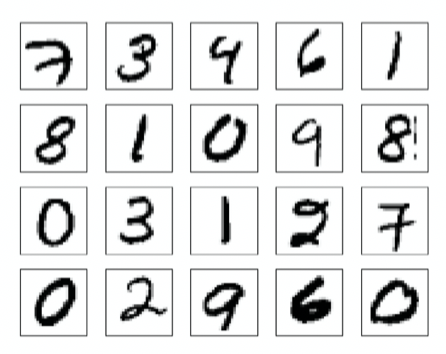
\includegraphics[scale=0.6]{fig2/C3/MNIST}%联邦学习的系统架构
	\caption{MNIST手写数字数据集}
	\label{fig:MNIST手写数字数据集}	
\end{figure}

我们让所有用户离线训练一个统一的卷积神经网络,以获得本地用户的加躁梯度。本地用户训练数据所采用的模型网络结构为一个包含两个卷积层和、两个池化层以及一个全连接层的CNN。模型的激活函数为ReLU,并引入了随机失活(Dropout正则)避免模型的果泥和。图\ref{fig:CNN模型网络结构}展示了CNN的网络结构。

\begin{figure}[!hbt]
\centering
	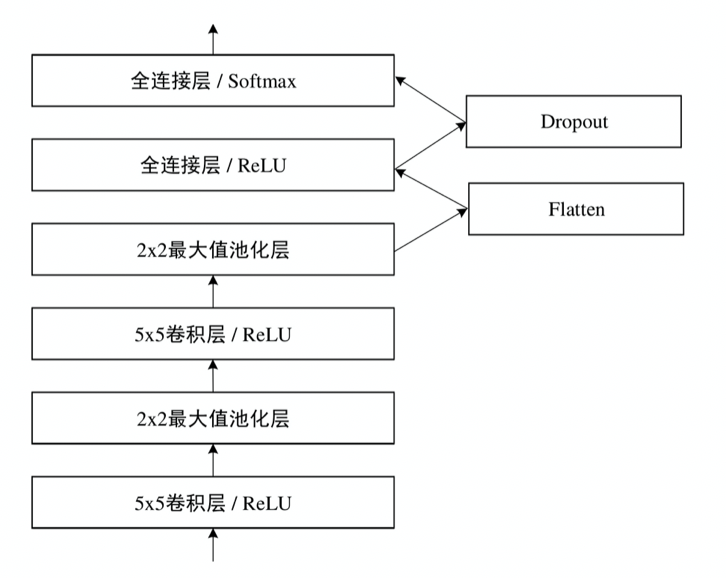
\includegraphics[scale=0.6]{fig2/C3/CNN网络结构}%联邦学习的系统架构
	\caption{模型网络结构}
	\label{fig:CNN模型网络结构}	
\end{figure}

所有的实验都是用PYTHON语言编译的,本文使用了TensorFlow-Federated,这是TensorFlow中的一个联邦学习库。我们使用Tensorflow去实现本地差分隐私算法,这是一个流行的深度学习库。我们在Python的基础上二次开发了该算法,并通过将该算法部署到多个边缘设备上构建了一个真实的联邦学习环境。以本地训练集MNIST为例,图\ref{fig:仿真联邦系统模型概览}展示了联邦学习的仿真模型概览。

\begin{figure}[!hbt]
\centering
	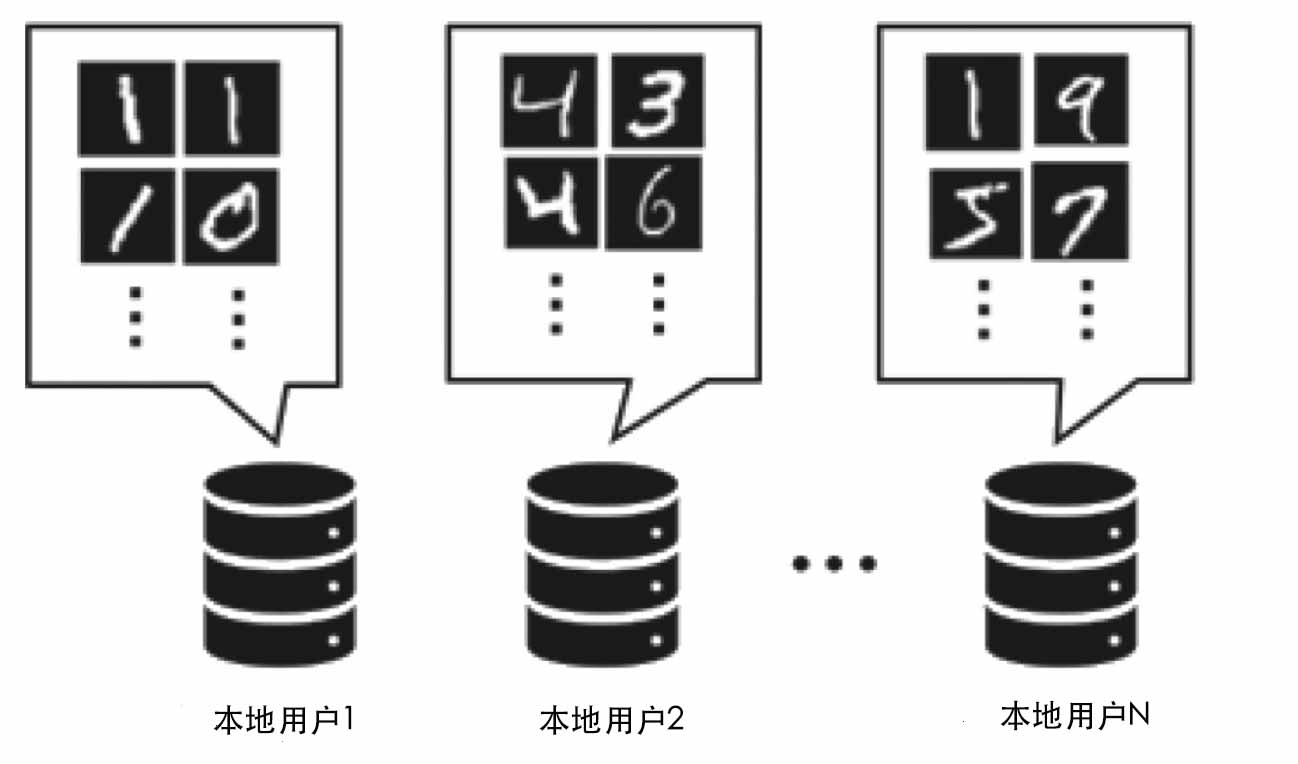
\includegraphics[scale=0.3]{fig2/C3/联邦系统仿真模型概览}%联邦学习的系统架构
	\caption{仿真联邦系统模型概览}
	\label{fig:仿真联邦系统模型概览}	
\end{figure}

\subsection{实验设计}
为了实现联邦学习的隐私保护,我们需要在本地训练的随机梯度下降算法中实现梯度的自适应扰动和裁剪,并采用MA机制跟踪每一次梯度扰动所增加的隐私预算。因此,代码的实现主要分为两个部分:梯度扰动和裁剪(Sanitizer),隐私预算跟踪(Accountant)。

图\ref{fig:实现本地自适应差分隐私的伪代码片段}展示了实现梯度扰动和裁剪、隐私预算跟踪的代码片段,为了实现整体算法满足$\epsilon$-差分隐私,Sanitizer需要完成以下三个步骤:首先,通过逐层关联传播算法计算神经元的贡献率和每批样本的梯度;其次,根据每个样本的梯度范数进行梯度裁剪以限制函数敏感度;最后,根据贡献率在梯度上添加自适应的噪声然后更新权重。

\begin{figure}[!hbt]
\centering
	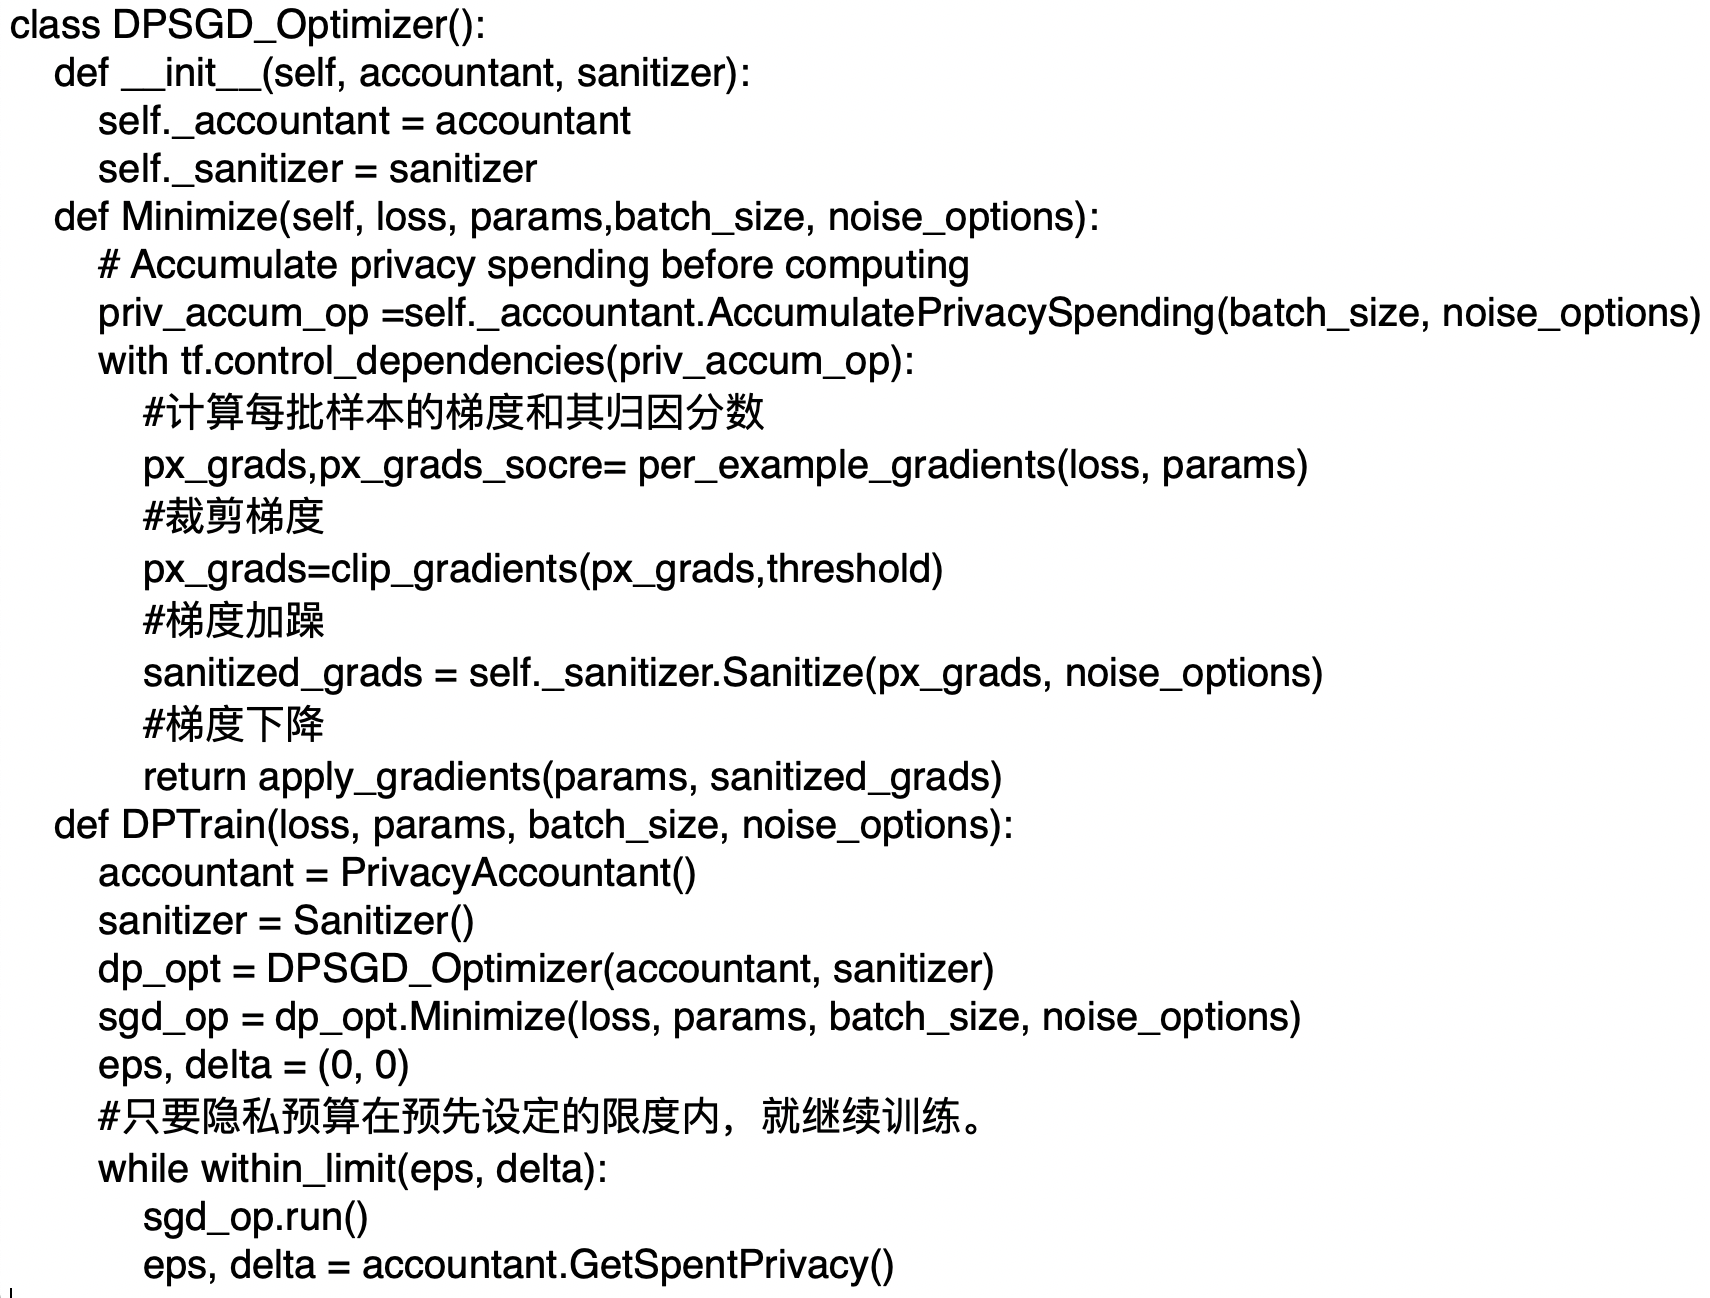
\includegraphics[scale=0.5]{fig2/C3/代码片段1}%联邦学习的系统架构
	\caption{实现本地自适应差分隐私的伪代码片段}
	\label{fig:实现本地自适应差分隐私的伪代码片段}	
\end{figure}

在TensorFlow中,由于性能原因,梯度计算是分批进行的,所以在训练过程,随机采样一批训练子样本$B$:
$\mathbf{g}_{B}=1 /|B| \sum_{x \in B} \nabla_{\theta} \mathcal{L}(\theta, x)$
。为了限制梯度更新的敏感度,我们需要计算每个批次的梯度$\nabla_{\theta} \mathcal{L}(\theta, x)$,具体由per\_example\_gradients函数实现。这样即使是大批量的训练,训练速度也不会大幅下降。在每个批次的训练中,我们会单独计算损失函数 
$\mathcal{L}$,也就是每个数据样本$x_{i}$都有单独的损失函数结果$\mathcal{L}$。一旦我们获得了每批数据样本的梯度,
我们可以很容易地使用TensorFlow操作符来对梯度进行裁剪,添加高斯噪声。

我们的实验主要分为三个部分:
\begin{enumerate}
\item [(1)] 针对本地自适应差分隐私SGD方案,分析噪声水平、裁剪阈值、隐藏层数量这些参数对模型分类准确率影响。
\item [(2)] 将本地自适应差分隐私SGD方案与非隐私的SGD、前人提出的差分隐私SGD方案(如表所示)进行对比,比较各个方案在相同隐私预算的情况下模型分类所能达到的准确率和模型收敛速度。
\item [(3)] 针对本地自适应差分隐私的联邦学习模型进行成员推理攻击进行实验,评估模型的隐私保护效用。

\begin{table}[H]
	\centering
	\begin{tabular}{cc}
		\hline
		基准方案名称& 具体算法\\
		\hline
		SGD& 没有实现差分隐私的随机梯度下降算法\\
		DP-SGD\upcite{ref57}& 在梯度上添加固定噪声大小的差分隐私随机梯度下降算法\\
		DS-SGD\upcite{ref67}& 在梯度下降过程中,选择性的进行参数共享实现隐私保护\\
		LDP-SGD& 本地差分隐私方案\\
		ADP-SGD& 我们的改进方案,使用梯度自适应加躁与裁剪\\
		\hline
	\end{tabular}
	\caption{本地自适应差分隐私与其他四种基准方案}
	\label{tab1}
\end{table}

\end{enumerate}

\subsection{结果分析}

\subsubsection{实验一(分析各个参数对模型准确率的影响)} 
分类模型的精度由多个因素决定,这些因素包括网络的拓扑结构、隐藏单元的数量以及模型训练的参数,如批量大小和学习率,必须仔细调整以获得最佳性能。有些参数是针对隐私的,如梯度范数裁剪阈值和噪声水平。本节实验重点研究噪声大小,梯度裁剪阈值和隐藏层数量这三种参数对于模型分类准确率的影响。为了准确的反映每种参数对于准确率的影响,我们控制变量的进行实验。参考值如下:1,000个隐藏层单元,600个批量,初始梯度范数裁剪阈值为4,初始的学习旅为0.1,在10个训练轮次之后线性衰减至0.051。噪声参数$\sigma$分别为2和5,用于训练CNN网络模型。对于每一种参数组合进行模型训练,直至隐私预算累积至$\left(2,10^{-5}\right)$-差分隐私。具体的实验结果如图\ref{fig:在MNIST数据集上噪声大小,裁剪阈值和隐藏层数量这三个参数对于训练准确率的影响}所示。

\begin{figure}[!hbt]
\centering
	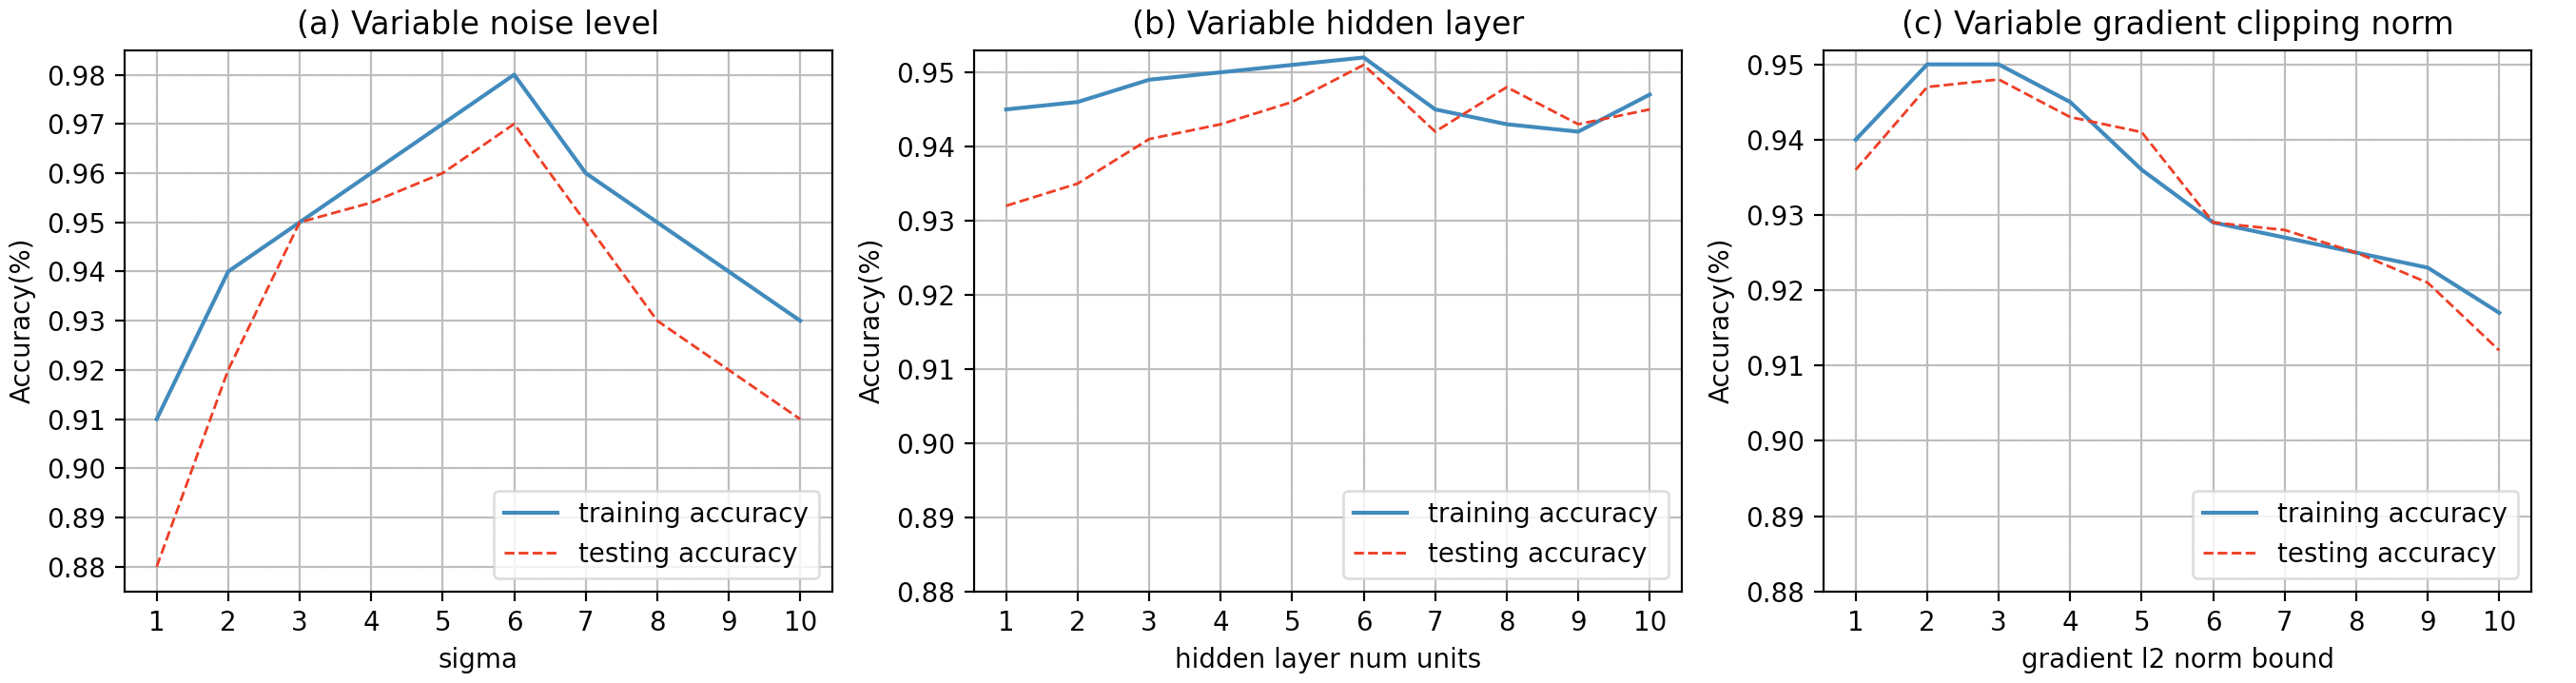
\includegraphics[scale=0.55]{fig2/C3/第三章实验一}%联邦学习的系统架构
	\caption{在MNIST数据集上噪声大小,裁剪阈值和隐藏层数量这三个参数对于训练准确率的影响}
	\label{fig:在MNIST数据集上噪声大小,裁剪阈值和隐藏层数量这三个参数对于训练准确率的影响}	
\end{figure}

如图\ref{fig:在MNIST数据集上噪声大小,裁剪阈值和隐藏层数量这三个参数对于训练准确率的影响}(a)展示的是噪声参数$\sigma$对模型准确率的影响,X轴是噪声水平,这个值的选择对准确性有很大影响。由于噪声参数$\sigma$与噪声采样的分布的方差是呈反比的,这意味着$\sigma$越大,添加的噪声量越小。通过添加更多的噪音,每轮训练步骤的隐私损失成比例缩小,所以我们可以在给定的累积隐私预算内运行更多的训练轮次。该模型在训练集和验证集上模型的准确率维持在88\%至98\%之间,我们的框架允许对梯度阈值进行自适应控制减少了过拟合情况,自适应的噪声添加根据训练轮次合理分配隐私预算,同时提高了模型的准确性和训练性能。

图\ref{fig:在MNIST数据集上噪声大小,裁剪阈值和隐藏层数量这三个参数对于训练准确率的影响}(b)展示了隐藏层数量对模型准确率的影响,X轴表示隐藏层单元数量。对于非差分隐私模型,更多的隐藏单元能有效避免过度拟合,因为更多的隐藏单元会让我们的训练更有针对性。然而,添加了差分隐私的模型训练,隐藏层数量的增加可能会影响梯度的敏感度,使每次梯度更新时添加更多的噪声。针对这个问题,我们的根据梯度的贡献率自适应添加噪声的方案能有效的控制敏感度有界,随着隐藏单位的数量增加,模型的准确率依然维持在93\%以上。

图\ref{fig:在MNIST数据集上噪声大小,裁剪阈值和隐藏层数量这三个参数对于训练准确率的影响}(c)展示了梯度范数裁剪阈值对模型准确率的影响,X轴表示梯度$\ell_{2}$-范数裁剪阈值$C^{0}$。当$C^{0}$为2-3时,模型准确率最高,接着随着$C^{0}$的增加,模型准确率逐渐降低至91\%左右,限制梯度范数会产生两个相反的效果:剪裁破坏了梯度估计的无偏性,如果剪裁参数太小,被剪切的平均梯度可能与真实梯度的方向大不相同。另一方面,增加裁剪阈值迫使我们在梯度中加入更多的噪声,也就是以$\sigma$$C^{0}$的比例添加噪声。而我们的自适应梯度裁剪方案能有效的考虑上一轮训练得到的梯度偏差和方差,取训练过程中未被剪辑的梯度范数的中值,模型准确率最高依然能达到95\%左右。

对于不同隐私预算的训练版本,我们用同样的网络架构进行了实验:一个包括1000个神经元的ReLU隐藏层,以及600个批量大小。为了限制敏感度,我们设置初始梯度范数裁剪阈值$C^{0}$为3。我们报告了四种隐私参数的训练结果,分别为小($\epsilon$=0.5)、中($\epsilon$=2)、大($\epsilon$=4)和更大($\epsilon$=8),固定$\delta=10^{-5}$,这里$\epsilon$代表训练神经网络的隐私保护水平。学习率最初设置为0.1,在10个训练回合后线性下降到0.052,然后固定为0.052。

\begin{figure}[!hbt]
\centering
	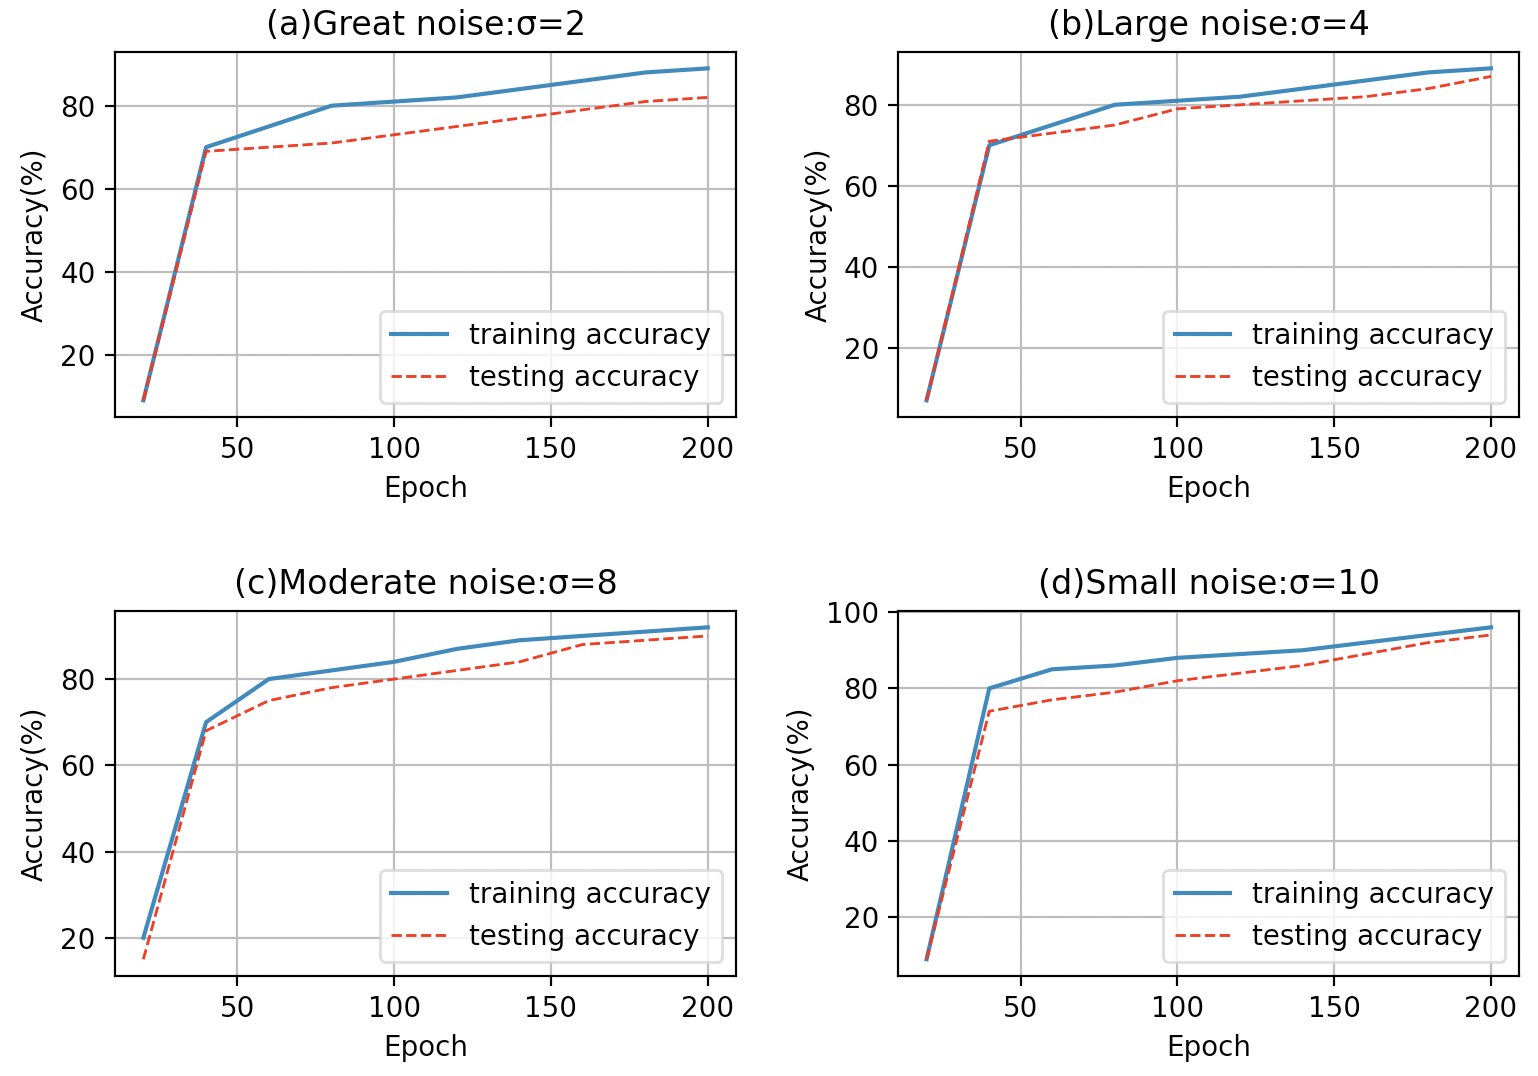
\includegraphics[scale=0.6]{fig2/C3/第三章实验一2}%联邦学习的系统架构
	\caption{在MNIST数据集上不同隐私预算下训练的准确率}
	\label{fig:在MNIST数据集上不同隐私预算下训练的准确率}	
\end{figure}

图\ref{fig:在MNIST数据集上不同隐私预算下训练的准确率}显示了不同隐私预算下的训练的结果,在每张图中,我们都显示了训练集和测试集上准确率的变化情况。对于隐私预算为$\left(0.5,10^{-5}\right)$,$\left(2,10^{-5}\right)$,$\left(4,10^{-5}\right)$和$\left(8,10^{-5}\right)$的差分隐私,分别达到81\%、94\%、95\%和97\%的测试集准确性。由图\ref{fig:在MNIST数据集上不同隐私预算下训练的准确率}(a)所示,当$\epsilon$=0.5时,由于给定的隐私预算较小,在训练的第30个轮次隐私预算消耗殆尽,模型基本趋近收敛,模型的准确率最高达到81\%。虽然在传统的差分隐私保护中,0<$\epsilon$<1时被认为能提供较强的隐私保护。而在联邦学习的深度神经网络中应用差分隐私时,由于网络的复杂性和训练多次大量迭代,导致隐私预算消耗的很快,0<$\epsilon$<1的取值会导致模型训练的精度大大下降。在深度学习方面应用差分隐私的大量研究表明,当0<$\epsilon$<=10时,能提供较强的隐私保护效果。如图\ref{fig:在MNIST数据集上不同隐私预算下训练的准确率}(b)(c)(d)所示,当$\epsilon$=2,4,8时,随着训练轮数的增加,模型均能达到收敛。我们的自适应差分隐私SGD方案,使模型在训练集和测试集上的准确度差异很小,这与理论上的观点一致,即添加噪声后的梯度训练依然有很好的泛化作用。相比之下,非差分隐私SGD的训练和测试准确率之间的差距随着训练轮次的增加而增加,容易造成过拟合。在噪声参数为$\left(8,10^{-5}\right)$时,模型在600个训练轮次后能达到接近非差分隐私模型的准确率。

\subsubsection{实验二(与前人的隐私保护方案进行对比实验)} 
我们将本文提出的本地自适应差分隐私方案(ADP-SGD)与SGD、DP-SGD、DS-SGD、LDP-SGD方案进行对比实验,选取的数据集为MNIST和CIFAR-10,网络模型为CNN5,具体的参数设置如下表所示。我们比较了不同方案在给定相同的隐私预算情况下,在测试集上所计算的目标函数的平均损失误差变化情况。

\begin{table}[H]
	\centering
	\begin{tabular}{ccc}
		\hline
		参数& MNIST& CIFAR-10\\
		\hline
		隐私预算$\epsilon$& 2/4& 2/4\\
		批大小& 600& 600\\
		初始梯度裁剪阈值& 3& 3\\
		学习率& 0.05& 0.05\\
		本地设备数量& 1000& 100\\
		训练轮数& 100& 100\\
		\hline
	\end{tabular}
	\caption{对比实验在数据集MNIST和CIFAR-10上的参数设置}
	\label{tab1}
\end{table}

图\ref{fig:不同隐私保护方案在MNIST数据集上训练的测试误差变化情况}显示了当隐私预算为$\left(2,10^{-5}\right)$,$\left(4,10^{-5}\right)$时,不同方案在MNIST和CIFAR-10数据集上平均损失误差随训练轮次的变化情况。

\begin{figure}[!hbt]
\centering
	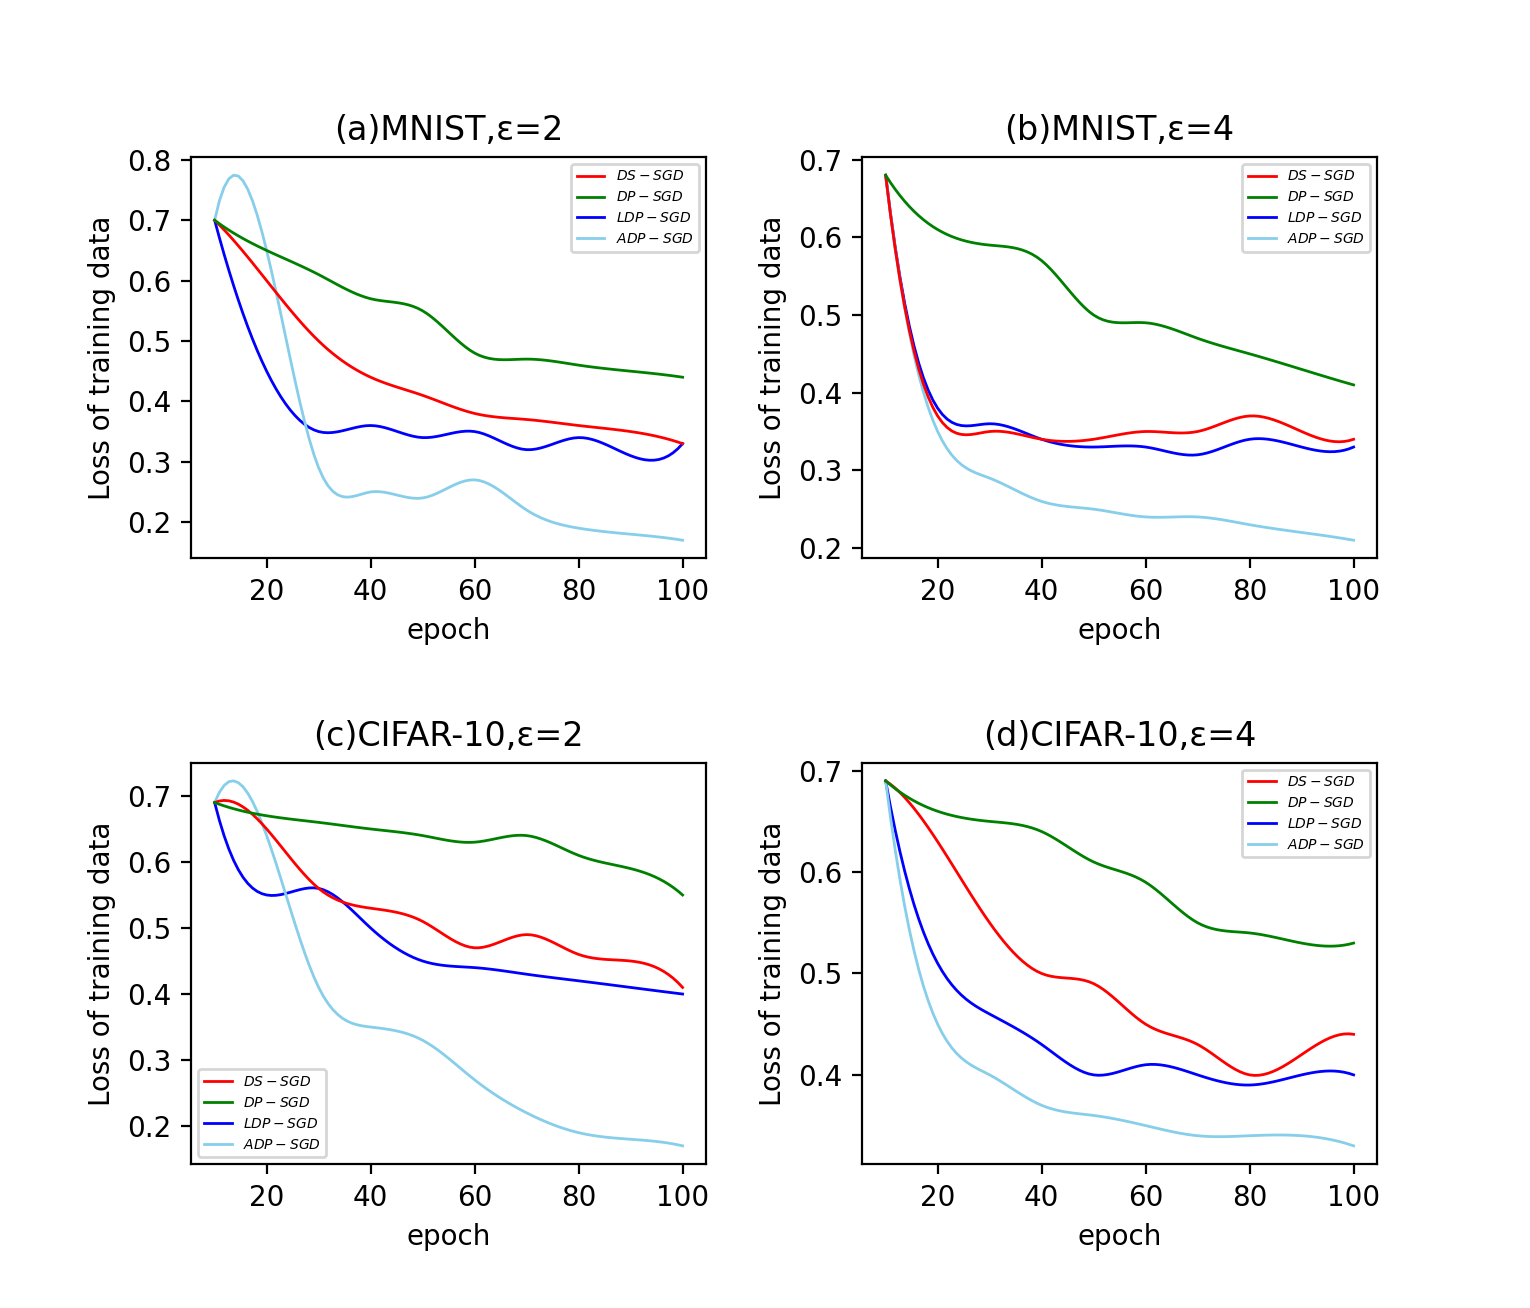
\includegraphics[scale=0.7]{fig2/C3/第三章对比实验}%联邦学习的系统架构
	\caption{不同隐私保护方案在MNIST数据集上训练的测试误差变化情况}
	\label{fig:不同隐私保护方案在MNIST数据集上训练的测试误差变化情况}	
\end{figure}

首先,对于MNIST数据集,在没有添加差分隐私保护的原始CNN模型上进行梯度下降训练,经过20个训练轮次后模型在训练集上得到的基准准确率为98.6\%,我们的方案(Adaptive Differential Privacy-SGD,ADP-SGD)在训练刚开始的一个轮次,训练集的训练误差下降较慢,这是由于刚开始训练时模型中所有梯度的归因分数较高,导致对于每个梯度分配的隐私预算较低,加躁后与原始值差异较大。然而,在20个轮次过后,模型收敛的速度远远超过其他三个基准差分隐私方案。在50个训练轮次之后,训练集的损失率降低至0.25以下,而DS-SGD和DP-SGD的训练损失值在10个轮次之后仅降低至0.35左右,DP-SGD更次之,在0.4左右。在相同的隐私预算下,ADP-SGD能在20个训练轮次后,梯度范数接近0.01且趋于平稳,意味着模型趋近收敛的速度最快。

其次,对于CIFAR-10数据集,由于图像本身复杂度的增加,在没有添加差分隐私保护的原始模型上进行梯度下降训练,经过20个训练轮次后模型在训练集上得到的基准准确率为97\%。LDP在前10个训练轮次的模型收敛速率最高,然而在第二个训练轮次过后,ADP-SGD达到35\%的模型准确率和0.05左右的梯度范数,训练数据损失值和梯度范数均比另外三个基准方案的效果优。

\begin{table}[H]
	\centering
	\begin{tabular}{ccc}
		\hline
		\diagbox{算法}{隐私预算}& $2,10^{-5}$& $4,10^{-5}$\\ %添加斜线表头
		\hline
		SGD& 98.6\%& 98.6\%\\
		DP-SGD& 88.9\%& 92.0\% \\
		DS-SGD& 91.4\%& 93.7\%\\
		LDP-SGD& 89.7\%& 91.3\%\\
		ADP-SGD& 94.6\%& 96.7\%\\
		\hline
	\end{tabular}
	\caption{本地自适应差分隐私与其他四种基准方案在100个训练轮次后模型所能达到的准确率}
	\label{本地自适应差分隐私与其他四种基准方案所能达到的模型精度}
\end{table}

表\ref{本地自适应差分隐私与其他四种基准方案所能达到的模型精度}显示了各个隐私保护方案在100个训练轮次过后所能达到的模型分类准确率。与非隐私的SGD方案相比,本文的自适应差分隐私SGD方案在提供隐私保护的前提下,模型准确率仅降低了2-4个百分点;在相同的隐私预算下,本文的方案相比于前人提出的隐私保护SGD算法对模型的准确率的影响更小。

综上,我们的方案在调整梯度自适应加躁和自适应裁剪后使得模型收敛率和准确率进一步提升,无论是在模型的准确率还是收敛速度方面都更加接近原始无隐私保护的模型。

\subsubsection{实验三(针对攻击模型,分析该方案的隐私保护效用)} 
我们曾在第一章介绍了针对联邦学习模型的隐私攻击,其中成员推理攻击是最流行的一类攻击,旨在确定一个输入样本x是否存在于模型训练集D中。攻击者可以是联邦学习的本地用户之一,也可以是中央服务器。由于深度学习模型对于“训练集中的数据”和“非训练集中的数据”通常会作出不同的行为反应,攻击者通过观察每条训练数据对损失函数的梯度的影响来判断该数据记录是否为目标模型的训练集成员,将成员推理攻击转换为二分类问题。攻击者在更新本地参数之前对目标数据点进行梯度上升,如果该数据记录是目标模型的成员数据,通过SGD的算法可以观察到梯度明显下降,成功推断出数据记录的成员属性。当攻击者作为本地用户参与全局模型的训练,攻击者可以观察到全局模型的更新,并通过注入对抗性的梯度样本,提取出被攻击者的训练数据集的信息。而当攻击者是中央服务器,它通过控制每个目标模型对全局模型更新的变化,提取出目标模型训练数据的分布信息,根据分布信息通过噪声生成数据。

我们重现了文献\upcite{ref70}中的成员推理攻击算法,配置和参数与之相同:目标模型采用卷积神经网络进行训练,数据集为MNIST。我们运行100个影子模型,每个模型通过逻辑回归算法进行训练。通过影子学习的技术构建与目标模型的训练数据相近的数据集。针对每一种数据样本,攻击者随机初始化一些数据记录作为影子模型的训练集数据。然后将此数据记录喂给目标模型得到预测向量,将所得的预测向量以及样本标签喂入攻击模型得到二分类的结果。

\begin{figure}[!hbt]
\centering
	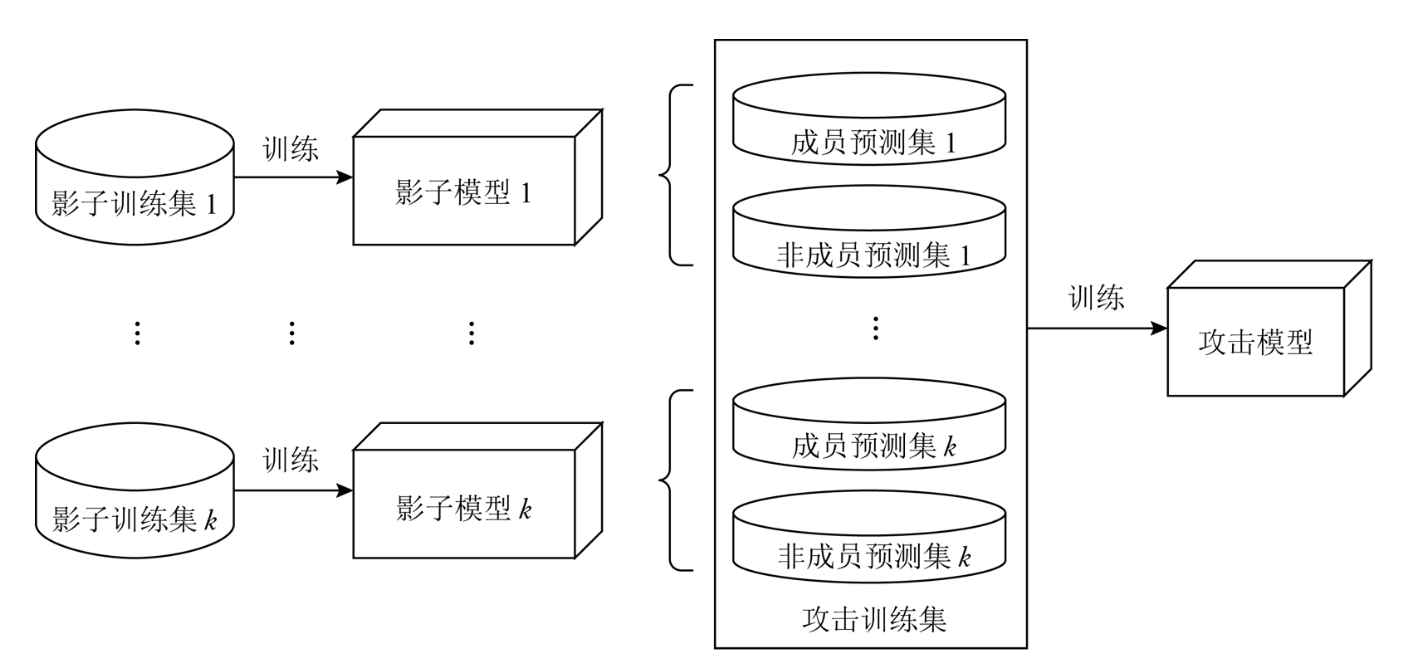
\includegraphics[scale=0.55]{fig2/C3/成员推理攻击}%联邦学习的系统架构
	\caption{成员推理攻击过程}
	\label{fig:成员推理攻击过程}	
\end{figure}

该实验的评估指标为攻击者的分类模型预测样本的准确率,它代表了模型的隐私保护效用。理论上在部署了差分隐私的联邦学习模型上进行成员推理攻击的准确率会下降。因此我们对比了在自适应差分隐私(隐私预算为$\epsilon=0.5$)和无隐私保护的模型上进行成员推理攻击的攻击准确率,结果如图\ref{fig:在不同模型上进行成员推理攻击的准确率}所示。

\begin{figure}[!hbt]
\centering
	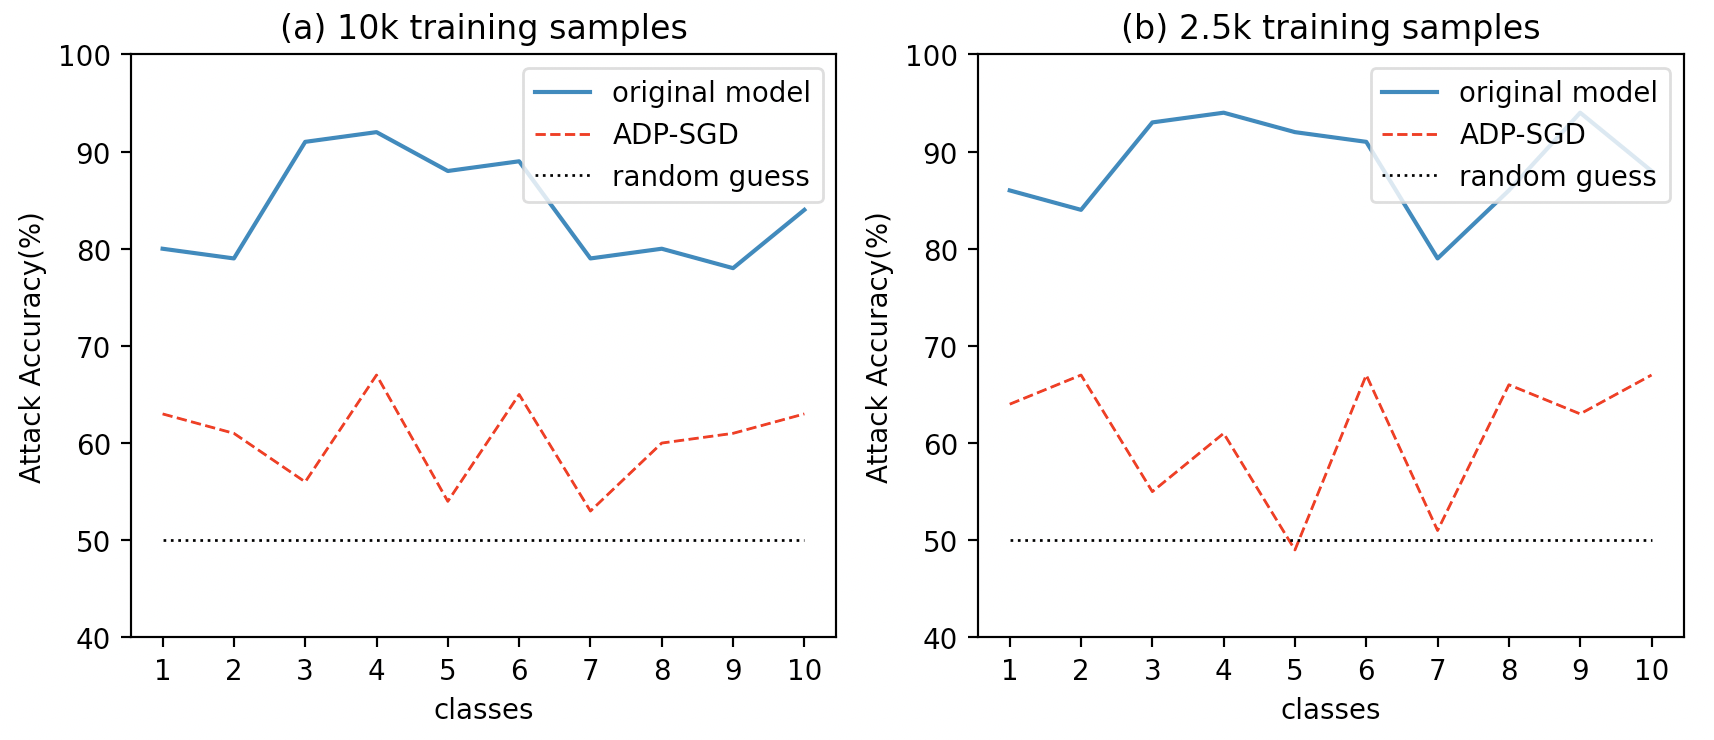
\includegraphics[scale=0.5]{fig2/C3/第三章实验三}%联邦学习的系统架构
	\caption{在不同模型上进行成员推理攻击的准确率}
	\label{fig:在不同模型上进行成员推理攻击的准确率}	
\end{figure}

我们分别在10k和2.5k个数据样本上进行攻击实验,图\ref{fig:在不同模型上进行成员推理攻击的准确率}中的(a)表示在10k数据样本上进行攻击实验,x轴表示对抗攻击的类别,蓝线(original model)表示在原始无隐私保护的模型上进行成员推理攻击的各个类别的攻击准确率,在不同类别上基本都可达到80\%~90\%的准确率。我们可以看到,敌手对识别包含在训练集中的样本有很高的置信值。当样本不在训练集中时,错误率相对较高。图\ref{fig:在不同模型上进行成员推理攻击的准确率}中的红线(ADP-SGD)显示了在添加了自适应差分隐私的模型上进行成员推理攻击的准确性。基准线是50\%(黑色虚线),这是敌手通过随机猜测达到的准确率。在应用差分隐私的情况下,敌手的推断准确率下降到50\%∼65\%,接近于随机猜测。这比原始模型的攻击准确率要低得多。而在2.5k的数据样本上进行攻击,我们的方案针对攻击实验能在5这个类别上将准确率降低至50\%左右,比随机猜测的准确率还要低,实验结果验证了本地自适应差分隐私算法的隐私保护效用。

\section{本章总结}
本章详细介绍了如何在联邦深度学习模型的本地训练算法中实现梯度的自适应加躁和裁剪。我们设计了一个自适应噪声添加的算法,在神经网络中,根据逐层传播算法计算神经元对于模型输出的贡献率,根据贡献率分配隐私预算,在梯度上注入高斯噪声。与传统的注入噪声的方法相比,通过噪声的自适应添加在相同的隐私保护程度下更好地提高了模型的准确性,并且证明了算法整体满足$(\epsilon, \delta)$-差分隐私。接着,本文设计了一种自适应调整梯度阈值的方案,通过计算梯度更新的方差和偏差,逐元素地对梯度进行裁剪,与之前的方案相比,通过使用梯度的自适应剪裁实现了相同的隐私保证,且加速了模型的收敛。之后我们利用“Moments Accountant”机制分析加噪累积产生的隐私预算,得到更精准的隐私损失分析。在实验部分。我们分别评估了各个参数对模型精度、收敛速度、隐私成本的影响以及方案的隐私保护效用,证明了我们的方案在相同的隐私保护程度下大大减少了噪声对模型输出结果的影响,与固定的梯度加躁和裁剪的方案相比提高了模型的准确性和收敛速度。

然而,当客户端在每次迭代中同时上传了大量的权重更新,中央云服务器仍然可以将它们链接在一起,推导出本地的训练参数信息。而且,当参与一次迭代的客户端数量达到上千人时,会导致聚合任务升级成一个高维任务,隐私预算暴增。因此,下一章我们对联邦学习模型框架进行了改进,在现有的联邦学习模型上新增混洗算法,实现联邦学习框架的隐私安全,结合隐私放大效应提高整体联邦学习的通信性能。



